% -*- LaTeX -*-

\documentclass[12pt,twoside]{article}
%\usepackage{titlesec,xr-hyper,healpix,graphicx,html,makeidx}
\usepackage{xr-hyper,healpix,graphicx,html,makeidx,dirtree}
%xr-hyper first to have correct Equation and Figure cross-referencing in html
%putting hyperref first screws up references in html
%%%
\usepackage{ae,lmodern}% load vectorial font, keep PDF small *and* good quality when in T1 font
\usepackage[T1]{fontenc}% underscore searchable in PDF, but larger PDF http://latex-community.org/forum/viewtopic.php?t=8891
\usepackage{tocloft} % to indent sections in TOC https://texblog.org/2011/09/09/10-ways-to-customize-tocloflot/
\begin{htmlonly}
% -*- LaTeX -*-
% This LaTeX file sets the Healpix version
% as it will appear in the documentation
% implement it with: % -*- LaTeX -*-
% This LaTeX file sets the Healpix version
% as it will appear in the documentation
% implement it with: % -*- LaTeX -*-
% This LaTeX file sets the Healpix version
% as it will appear in the documentation
% implement it with: \input{hpxversion}
% \newcommand{\hpxversion}{3.31}
% \newcommand{\hpxverstex}{3\_31}
% \newcommand{\hpxversion}{3.40}
% \newcommand{\hpxverstex}{3\_40}
% \newcommand{\hpxversion}{3.41}
% \newcommand{\hpxverstex}{3\_41}
\newcommand{\hpxversion}{3.50}
\newcommand{\hpxverstex}{3\_50}

% \newcommand{\hpxversion}{3.31}
% \newcommand{\hpxverstex}{3\_31}
% \newcommand{\hpxversion}{3.40}
% \newcommand{\hpxverstex}{3\_40}
% \newcommand{\hpxversion}{3.41}
% \newcommand{\hpxverstex}{3\_41}
\newcommand{\hpxversion}{3.50}
\newcommand{\hpxverstex}{3\_50}

% \newcommand{\hpxversion}{3.31}
% \newcommand{\hpxverstex}{3\_31}
% \newcommand{\hpxversion}{3.40}
% \newcommand{\hpxverstex}{3\_40}
% \newcommand{\hpxversion}{3.41}
% \newcommand{\hpxverstex}{3\_41}
\newcommand{\hpxversion}{3.50}
\newcommand{\hpxverstex}{3\_50}

% -*- LaTeX -*-
% This LaTeX file sets the IDL version required to run Healpix-DL
% as it will appear in the documentation
% implement it with: % -*- LaTeX -*-
% This LaTeX file sets the IDL version required to run Healpix-DL
% as it will appear in the documentation
% implement it with: % -*- LaTeX -*-
% This LaTeX file sets the IDL version required to run Healpix-DL
% as it will appear in the documentation
% implement it with: \input{idlversion}
%\newcommand{\idlversion}{5.6 }
%\newcommand{\idlversion}{6.0 }
\newcommand{\idlversion}{6.1 }

%\newcommand{\idlversion}{5.6 }
%\newcommand{\idlversion}{6.0 }
\newcommand{\idlversion}{6.1 }

%\newcommand{\idlversion}{5.6 }
%\newcommand{\idlversion}{6.0 }
\newcommand{\idlversion}{6.1 }

% -*- LaTeX -*-
% This LaTeX file sets the GDL version required to run Healpix-IDL
% as it will appear in the documentation
% implement it with: % -*- LaTeX -*-
% This LaTeX file sets the GDL version required to run Healpix-IDL
% as it will appear in the documentation
% implement it with: % -*- LaTeX -*-
% This LaTeX file sets the GDL version required to run Healpix-IDL
% as it will appear in the documentation
% implement it with: \input{gdlversion}
% \newcommand{\gdlversion}{0.9rc3 }
% \newcommand{\gdlversion}{0.9.2 }
% \newcommand{\gdlversion}{0.9.3 }
% \newcommand{\gdlversion}{0.9.6 }% Jan 2016
% \newcommand{\gdlversion}{0.9.7 }% Jan 2017
\newcommand{\gdlversion}{0.9.8}% Mar 2018
\newcommand{\gdlreldate}{March 2018}
\newcommand{\gdlsite}{https://github.com/gnudatalanguage/gdl}

% \newcommand{\gdlversion}{0.9rc3 }
% \newcommand{\gdlversion}{0.9.2 }
% \newcommand{\gdlversion}{0.9.3 }
% \newcommand{\gdlversion}{0.9.6 }% Jan 2016
% \newcommand{\gdlversion}{0.9.7 }% Jan 2017
\newcommand{\gdlversion}{0.9.8}% Mar 2018
\newcommand{\gdlreldate}{March 2018}
\newcommand{\gdlsite}{https://github.com/gnudatalanguage/gdl}

% \newcommand{\gdlversion}{0.9rc3 }
% \newcommand{\gdlversion}{0.9.2 }
% \newcommand{\gdlversion}{0.9.3 }
% \newcommand{\gdlversion}{0.9.6 }% Jan 2016
% \newcommand{\gdlversion}{0.9.7 }% Jan 2017
\newcommand{\gdlversion}{0.9.8}% Mar 2018
\newcommand{\gdlreldate}{March 2018}
\newcommand{\gdlsite}{https://github.com/gnudatalanguage/gdl}

% -*- LaTeX -*-
% This LaTeX file sets the FL version required to run Healpix-IDL
% as it will appear in the documentation
% implement it with: % -*- LaTeX -*-
% This LaTeX file sets the FL version required to run Healpix-IDL
% as it will appear in the documentation
% implement it with: % -*- LaTeX -*-
% This LaTeX file sets the FL version required to run Healpix-IDL
% as it will appear in the documentation
% implement it with: \input{flversion}
%\newcommand{\flversion}{0.79.40 }% May 2017
%\newcommand{\flversion}{0.79.41 }% ?? 2017
%\newcommand{\flversion}{0.79.43.1 }% Jan 2018
\newcommand{\flversion}{0.79.44 }% Apr 2018
\newcommand{\flsitea}{https://www.flxpert.hu/fl}
\newcommand{\flsiteb}{http://85.255.9.75/fl}


%\newcommand{\flversion}{0.79.40 }% May 2017
%\newcommand{\flversion}{0.79.41 }% ?? 2017
%\newcommand{\flversion}{0.79.43.1 }% Jan 2018
\newcommand{\flversion}{0.79.44 }% Apr 2018
\newcommand{\flsitea}{https://www.flxpert.hu/fl}
\newcommand{\flsiteb}{http://85.255.9.75/fl}


%\newcommand{\flversion}{0.79.40 }% May 2017
%\newcommand{\flversion}{0.79.41 }% ?? 2017
%\newcommand{\flversion}{0.79.43.1 }% Jan 2018
\newcommand{\flversion}{0.79.44 }% Apr 2018
\newcommand{\flsitea}{https://www.flxpert.hu/fl}
\newcommand{\flsiteb}{http://85.255.9.75/fl}


% -*- LaTeX -*-
% This LaTeX file sets the healpy version
% as it will appear in the documentation
% implement it with: % -*- LaTeX -*-
% This LaTeX file sets the healpy version
% as it will appear in the documentation
% implement it with: % -*- LaTeX -*-
% This LaTeX file sets the healpy version
% as it will appear in the documentation
% implement it with: \input{hpyversion}
% \newcommand{\hpyversion}{1.12.0 }
% \newcommand{\hpyversion}{1.12.4 }
\newcommand{\hpyversion}{1.12.5 }
\newcommand{\hpysite}{https://github.com/healpy/healpy}

% \newcommand{\hpyversion}{1.12.0 }
% \newcommand{\hpyversion}{1.12.4 }
\newcommand{\hpyversion}{1.12.5 }
\newcommand{\hpysite}{https://github.com/healpy/healpy}

% \newcommand{\hpyversion}{1.12.0 }
% \newcommand{\hpyversion}{1.12.4 }
\newcommand{\hpyversion}{1.12.5 }
\newcommand{\hpysite}{https://github.com/healpy/healpy}

% file read by healpix.perl and healpix.sty to determine HEALPix source URL
%srcurl = https://sourceforge.net/p/healpix/code/HEAD/tree/trunk/
%\newcommand{\srcurl}{https://sourceforge.net/p/healpix/code/HEAD/tree/trunk/}
\newcommand{\srcurl}{https://healpix.sourceforge.io/src/\hpxversion/}







% -*- LaTeX -*-
% This LaTeX file sets the Healpix websites
% as they will appear in the documentation
% implement it with: % -*- LaTeX -*-
% This LaTeX file sets the Healpix websites
% as they will appear in the documentation
% implement it with: % -*- LaTeX -*-
% This LaTeX file sets the Healpix websites
% as they will appear in the documentation
% implement it with: \input{hpxwebsites}

% -------- mailing list
\newcommand{\healpixmail}{{\em healpix-support} \texttt{at} {\em lists.sourceforge.net}}

% -------- source web site: see healpix_src_url.tex

% -------- doc web site
\newcommand{\hpxwebsite}{https://healpix.sourceforge.io}
\newcommand{\oldhpxwebsite}{http://healpix.sf.net}

% --------- used in install.tex:
%\newcommand{\healpixwebpage}{\oldhpxwebsite}
\newcommand{\healpixwebpage}{\hpxwebsite}
\newcommand{\healpixsupport}{\healpixwebpage/support.php}

% DO NOT FORGET TO UPDATE main.html AS WELL !!!!!


%--------------------- web site(s) showing on front page
% %OLD
% \newcommand{\defwebsite}{\website{\htmladdnormallink{\oldhpxwebsite}{\oldhpxwebsite}}}

%TRANSITION
\newcommand{\defwebsite}{\website{\htmladdnormallink{\hpxwebsite}{\hpxwebsite}\\\htmladdnormallink{\oldhpxwebsite}{\oldhpxwebsite}}}

% %FUTURE
% \newcommand{\defwebsite}{\website{\htmladdnormallink{\hpxwebsite}{\hpxwebsite}}}




% -------- mailing list
\newcommand{\healpixmail}{{\em healpix-support} \texttt{at} {\em lists.sourceforge.net}}

% -------- source web site: see healpix_src_url.tex

% -------- doc web site
\newcommand{\hpxwebsite}{https://healpix.sourceforge.io}
\newcommand{\oldhpxwebsite}{http://healpix.sf.net}

% --------- used in install.tex:
%\newcommand{\healpixwebpage}{\oldhpxwebsite}
\newcommand{\healpixwebpage}{\hpxwebsite}
\newcommand{\healpixsupport}{\healpixwebpage/support.php}

% DO NOT FORGET TO UPDATE main.html AS WELL !!!!!


%--------------------- web site(s) showing on front page
% %OLD
% \newcommand{\defwebsite}{\website{\htmladdnormallink{\oldhpxwebsite}{\oldhpxwebsite}}}

%TRANSITION
\newcommand{\defwebsite}{\website{\htmladdnormallink{\hpxwebsite}{\hpxwebsite}\\\htmladdnormallink{\oldhpxwebsite}{\oldhpxwebsite}}}

% %FUTURE
% \newcommand{\defwebsite}{\website{\htmladdnormallink{\hpxwebsite}{\hpxwebsite}}}




% -------- mailing list
\newcommand{\healpixmail}{{\em healpix-support} \texttt{at} {\em lists.sourceforge.net}}

% -------- source web site: see healpix_src_url.tex

% -------- doc web site
\newcommand{\hpxwebsite}{https://healpix.sourceforge.io}
\newcommand{\oldhpxwebsite}{http://healpix.sf.net}

% --------- used in install.tex:
%\newcommand{\healpixwebpage}{\oldhpxwebsite}
\newcommand{\healpixwebpage}{\hpxwebsite}
\newcommand{\healpixsupport}{\healpixwebpage/support.php}

% DO NOT FORGET TO UPDATE main.html AS WELL !!!!!


%--------------------- web site(s) showing on front page
% %OLD
% \newcommand{\defwebsite}{\website{\htmladdnormallink{\oldhpxwebsite}{\oldhpxwebsite}}}

%TRANSITION
\newcommand{\defwebsite}{\website{\htmladdnormallink{\hpxwebsite}{\hpxwebsite}\\\htmladdnormallink{\oldhpxwebsite}{\oldhpxwebsite}}}

% %FUTURE
% \newcommand{\defwebsite}{\website{\htmladdnormallink{\hpxwebsite}{\hpxwebsite}}}



\end{htmlonly}

\hypersetup{%
	pdftitle={HEALPix Installation Guidelines},%
	pdfauthor={E. Hivon et al},%
	pdfkeywords={HEALPix, Installation},%
	colorlinks=true}


\newcommand{\nside}{N_{\mathrm{side}}}
\newcommand{\npix}{N_{\mathrm{pix}}}
\newcommand{\lmax}{\ell_{\mathrm{max}}}
\newcommand{\doubledash}{\latexhtml{-{}-}{-{}--}}
\renewcommand{\contentsname}{{TABLE OF CONTENTS}}

% in LaTeX2HTML:
% \hyperref{HTML text}{PDF text1}{PDF text2}{label}
% in PDFTeX:
% \hyperref{URL}{cat}{name}{text}
%
% command for external link
\newcommand{\linklatexhtml}[3]{% \linklatexhtml{name}{latex_target}{html_target}
\latexhtml{\htmladdnormallink{#1}{#2}}{\htmladdnormallink{#1}{#3}}}
% commands for arbitrary link
\newcommand{\mylink}[2]{% \mylink{link_id}{link_text} (internal link)
\latexhtml{\hyperlink{#1}{#2}}{\hyperref{#2}{}{}{#1}}}
\newcommand{\mylinkext}[2]{% \mylink{link_id}{link_text}  (external link)
\latexhtml{\htmlref{#2}{#1}}{\hyperref{#2}{}{}{#1}}}
%\latexhtml{\hyperref[#1]{#2}}{\hyperref{#2}{}{}{#1}}}
%\latexhtml{\hyperref{#2}{}{}{#1}}{\hyperref{#2}{}{}{#1}}}

% \newcommand{\mylink}[2]{% \mylink{link_id}{link_text}
% \latexhtml{\hyperlink{#1}{#2}}{\htmlref{#2}{#1}}}
% \newcommand{\mylink}[2]{% \mylink{link_id}{link_text}
% \latexhtml{\hyperref{#1}{}{}{#2}}{\hyperref{#2}{}{}{#1}}}

% commands for targets 
% http://tex.stackexchange.com/questions/17057/hypertarget-seems-to-aim-a-line-too-low
\makeatletter
     \newcommand{\nop}[1]{\Hy@raisedlink{\hypertarget{#1}{}}}
\makeatother
\newcommand{\mytarget}[1]{\nop{#1}}%    \mytarget{id}
\begin{htmlonly}
 \newcommand{\mytarget}[1]{\label{#1}}
\end{htmlonly}
% \newcommand{\crossref}[3]{% \crossref{text}{latex_target}{html_target}
% \latexhtml{\htmlref{#1}{#2}}{%
% \htmladdnormallink{#1}{#3}}}
% \newcommand{\crossref}[3]{% \crossref{text}{latex_target}{html_target}
% \latexhtml{\htmlref{#1}{#2}}{%
% \htmlref{#1}{#2}}}
%%%%%\externalref{#1}{#2}}}

%\begin{latexonly}
%\end{latexonly}

%\input psfig

\sloppy
\setcounter{secnumdepth}{10}%must be non-zero for cross-reference of Figs and Sections
\setcounter{tocdepth}{10}
\newcounter{append}
%\newcounter{figure}
%\newcounter{tab}

% CROSS-LINK
%%%%http://tex.stackexchange.com/questions/41539/does-hyperref-work-between-two-files
%% add xr-hyper (part of hyperref) to used packages, *BEFORE* hyperref (or html)
\newcommand{\facname}{} % must be here because it is in idl.tex
\newcommand{\FACNAME}{} % must be here because it is in idl.tex
\externaldocument{intro}[intro.pdf]
%\externaldocument{install}[install.pdf]
\externaldocument{csub}[csub.pdf]
\externaldocument{idl}[idl.pdf]
\externaldocument{facilities}[facilities.pdf]
\externaldocument{subroutines}[subroutines.pdf]
\begin{htmlonly}
\externallabels{.}{/tmp/introlabels.pl}
\externallabels{.}{/tmp/intro_labels.pl}
%\externallabels{.}{/tmp/installlabels.pl}
\externallabels{.}{/tmp/csublabels.pl}
\externallabels{.}{/tmp/csub_labels.pl}
\externallabels{.}{/tmp/idllabels.pl}
\externallabels{.}{/tmp/idl_labels.pl}
\externallabels{.}{/tmp/facilitieslabels.pl}
\externallabels{.}{/tmp/fac_labels.pl}
\externallabels{.}{/tmp/subroutineslabels.pl}
\externallabels{.}{/tmp/sub_labels.pl}
\end{htmlonly}

%%%%%
\begin{document}

\title{\healpix Facility Installation Guidelines}
\docid{INSTALLATION GUIDE} 
\docrv{Version \hpxversion}
\author{Eric Hivon, Anthony J.~Banday, Matthias Bartelmann, Benjamin D.~Wandelt,
Frode K.~Hansen and Krzysztof M.~G\'orski}
\abstract{This document describes the installation for the \healpix facilities.}
%% -*- LaTeX -*-
% This LaTeX file sets the Healpix website
% as it will appear in the documentation
% implement it with: % -*- LaTeX -*-
% This LaTeX file sets the Healpix website
% as it will appear in the documentation
% implement it with: % -*- LaTeX -*-
% This LaTeX file sets the Healpix website
% as it will appear in the documentation
% implement it with: \input{hpxwebsite}
%
% DEPRECATED !!!! replaced with hpxwebsites.tex
%

%
% DEPRECATED !!!! replaced with hpxwebsites.tex
%

%
% DEPRECATED !!!! replaced with hpxwebsites.tex
%

%\website{\hpxws}
\defwebsite
\date{\today}

\frontpage
\tableofcontents
\newpage

\section{Introduction}

In this document the installation procedure for the \healpix
distribution is outlined. \healpix comprises a suite of Fortran 90, C++, 
IDL, Java and Python routines
providing both stand-alone facilities and callable subroutines as an alternative
for those users who wish to build their own tools.
A set of C subroutines and functions is also provided. 

The distribution can be downloaded as a gzipped tarred file, {\em or} as a zipped file,
which can respectively be unpacked by executing the commands\footnote{Microsoft Windows users can have a look at \\
\url{https://sourceforge.net/p/healpix/wiki/Windows\%20and\%20peazip/}} \hfill\newline
%\begin{verbatim}
\texttt{\% gunzip Healpix\_\hpxversion.tar.gz}\hfill\\
\texttt{\% tar -xpf Healpix\_\hpxversion.tar}\hfill\\
or \hfill\\
\texttt{\% tar -xzpf Healpix\_\hpxversion.tar.gz}\hfill\\
or \hfill\\
\texttt{\% unzip Healpix\_\hpxversion.zip}\hfill\\
%\end{verbatim}
creating a directory named \texttt{Healpix\_\hpxversion}\ whose structure is shown in Figure
\ref{fig:dirtree}.


\begin{figure}[!ht]
\latexhtml{%for latex
% cf extratbb -vO image_file
\centerline{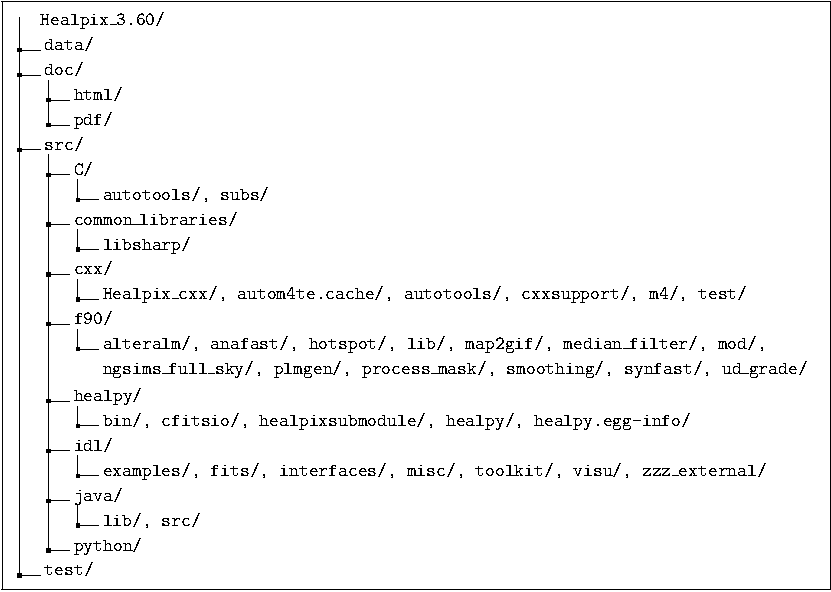
\includegraphics[bb=0 0 418 284,width=\textwidth,clip]{fig/new_dir_tree.pdf}}
}{%for html
\centerline{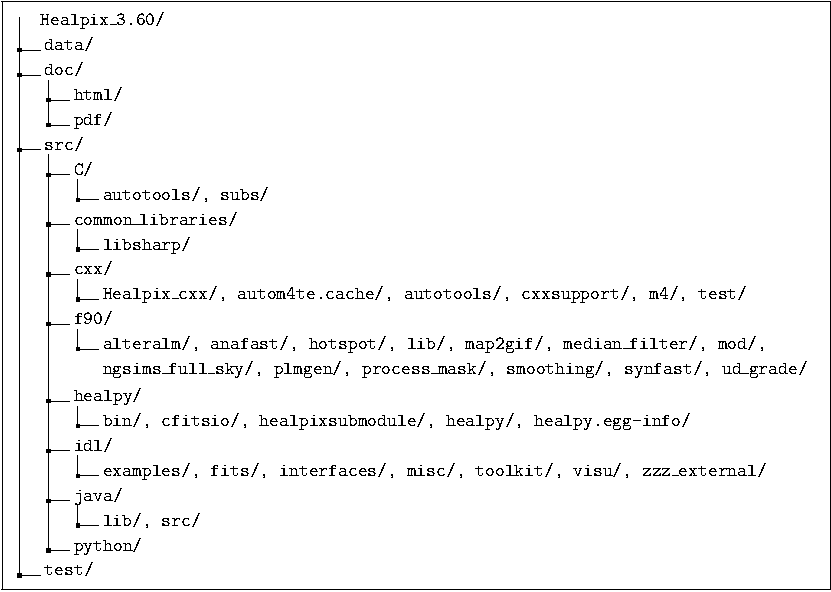
\includegraphics[]{fig/new_dir_tree}}% %\centerline{\psfig{figure=fig/dir_tree.eps,width=\textwidth}}
% \latexhtml{%for latex
% % cf extratbb -vO image_file
% %\centerline{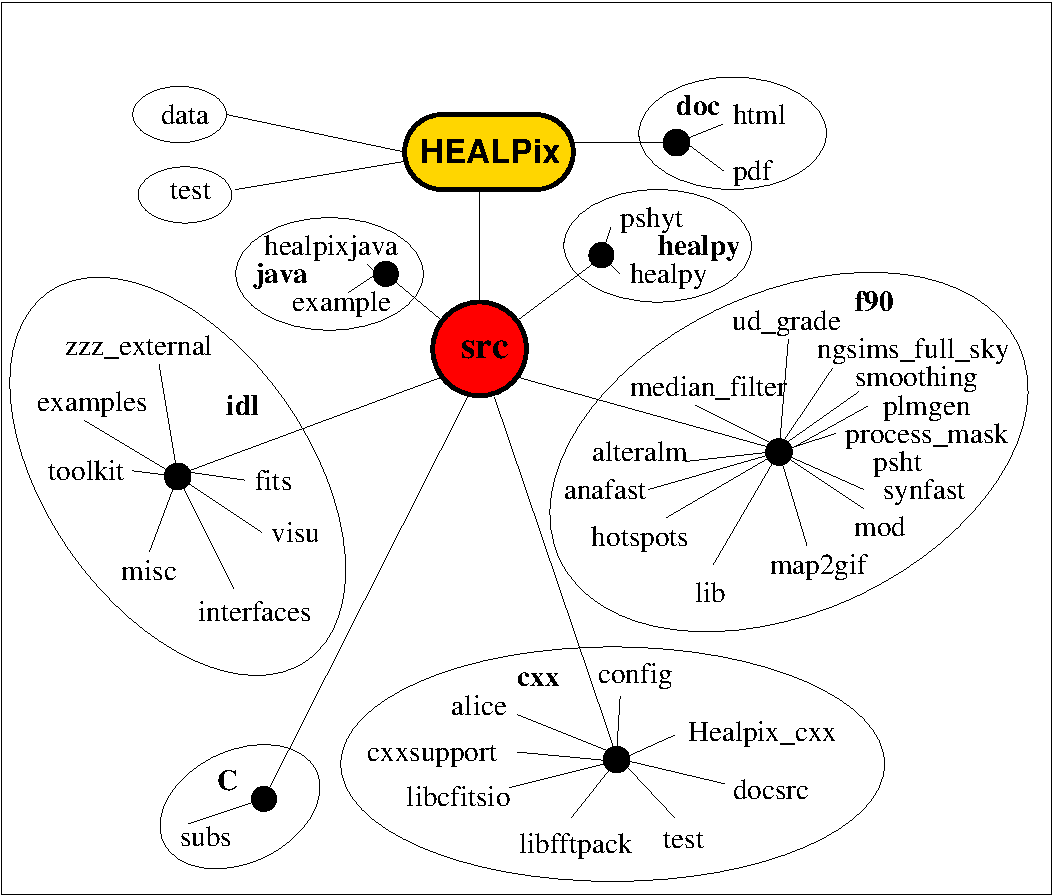
\includegraphics[bb=0pt 0pt 562pt 478pt,width=\textwidth,clip]{fig/dir_tree.pdf}}
% \centerline{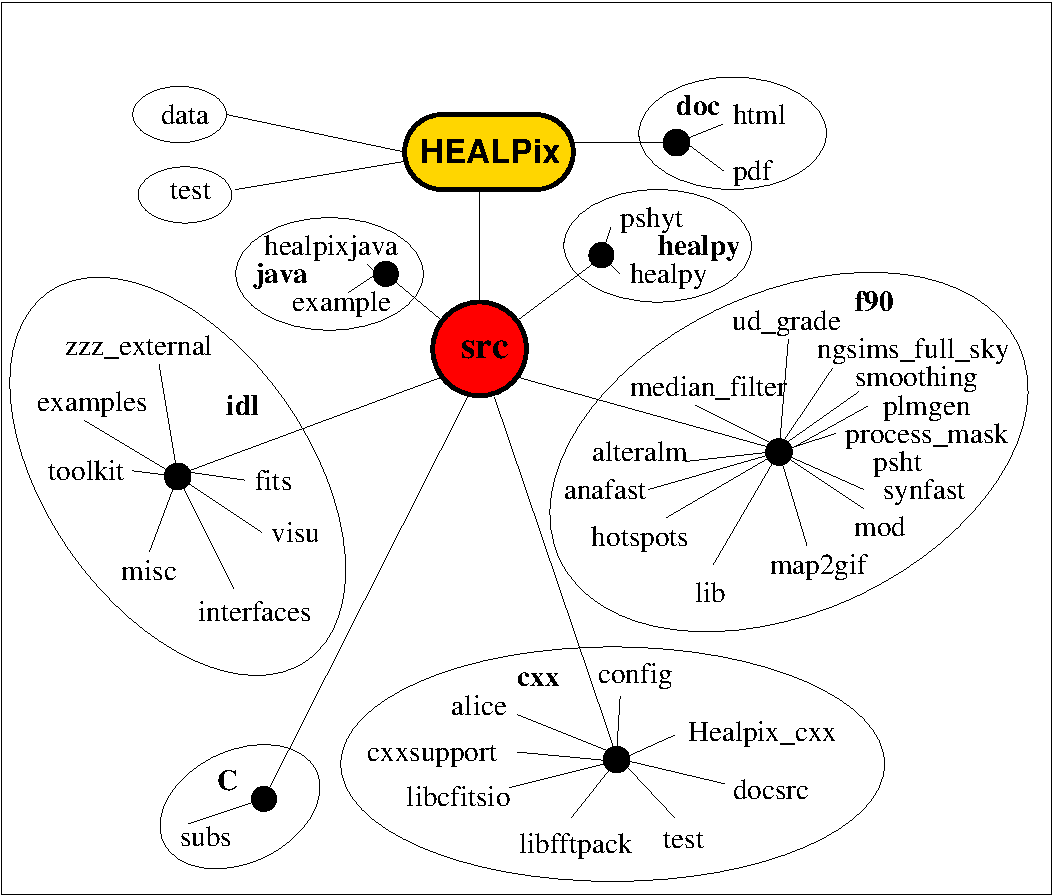
\includegraphics[bb=0 0 506 430,width=\textwidth,clip]{fig/dir_tree.pdf}}
% }{%for html
% \centerline{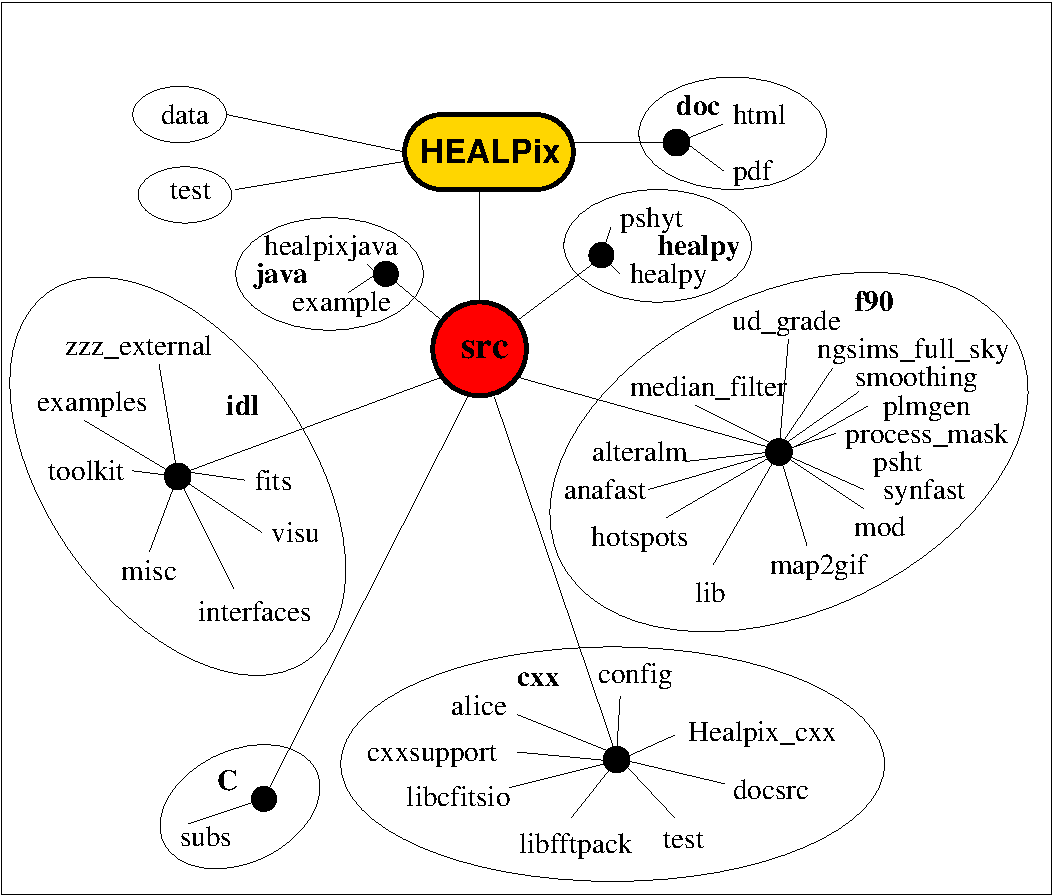
\includegraphics[width=0.5\textwidth]{fig/dir_tree}}
}
\caption[Directory structure]{%
\label{page:dirtree}
\label{fig:dirtree} % put \label *IN* \caption !!!!!
The directory structure for the \healpix distribution. }
\end{figure}

As with most freely available software, the distribution
comes with caveats, the major one being that although we have attempted
to automate the installation as much as possible, not all eventualities
can ever be foreseen. We have tested the installation on the following 
platforms: \hfill\newline
\noindent AIX, IRIX, IRIX64, Linux, SunOS, ALPHA and Darwin (MacOS) \hfill\newline

There may be problems in the facility build due to the local system 
configuration which is beyond our control. 


\section{Installation Requirements}
\label{sec:requirements}


%--------------------------------------------------------------------
\begin{table}[!h]
\begin{tabular}{p{0.15\hsize} p{0.35\hsize} p{0.4\hsize}} \hline  
  \textbf{Healpix Package} & \textbf{Information on installation} &
\textbf{Information on routines}\\ \hline
                            &                      &     \\ %%% for presentation
%
  Fortran 90     & This document & 
\linklatexhtml{"Fortran Facilities"}{facilities.pdf}{facilities.htm} and 
\linklatexhtml{"Fortran Subroutines"}{subroutines.pdf}{subroutines.htm} documents \\
%
 & & \\
%
  IDL/GDL/FL        & This document  & 
\linklatexhtml{"IDL Facilities"}{idl.pdf}{idl.htm}\\
 & & \\
%
  C++     & This document & 
%  C++     & This document, or \phantom{filling up --} \texttt{src/cxx/README.compilation} & 
%\htmladdnormallink{"C++ Facilities and Subroutines"}{index_cxx.html}
\linklatexhtml{"C++ Facilities and Subroutines"}{../html/index_cxx.html}{index_cxx.html}
 (HTML only)\\
%
 & & \\
%
  C       & This document, or \phantom{filling up --} \texttt{src/C/README} & 
    \linklatexhtml{"C Subroutines Overview"}{csub.pdf}{csub.htm} \\ 
%
 & & \\
%
  Java    & \texttt{src/java/README} & 
%\htmladdnormallink{"Java Overview"}{java/index.html}
\linklatexhtml{"Java Overview"}{../html/java/index.html}{java/index.html}
 (HTML only)\\
%
 & & \\
%
  Python    & This document, or \phantom{filling up --} \texttt{src/healpy/INSTALL} & 
\linklatexhtml{"Healpy
Documentation"}{https://healpy.readthedocs.io/en/latest}{https://healpy.readthedocs.io/en/latest}
 (HTML only)\\
%
                                   &                          \\ \hline %%% for presentation
\end{tabular}
\caption[Documentation]{%
\label{tab:allpackages}  % put \label *IN* \caption !!!!!
Documentation on the installation and usage of the different packages}
\end{table}
%--------------------------------------------------------------------

The major part of the \healpix distribution is written in both \textbf{Fortran 90} and \textbf{C++} and
so the appropriate compiler(s) must be present (Linux and Darwin users should look
at Section~\ref{sec:freef90compilers} about free F90 compilers. Microsoft Windows
users should look at Section~\ref{sec:windows}). Many visualisation tools and map
manipulation routines are provided in \textbf{IDL} (please note 
that at least version \idlversion is required), \textbf{Java} and \textbf{Python}. Some of the \healpix routines are
also available in \textbf{C}. \\
Starting with version 3.0, the
\linklatexhtml{healpy}{\gdlsite}{\gdlsite}
(HEALPix in \textbf{Python}) library has been integrated into \healpix releases. Since it
is, to a large extent, a
wrapper to the C++ routines, installing it also requires a C++ compiler (on top
of \texttt{python} and a few supporting Python libraries) but it will perform
its own compilation of the current \healpix C++ library.\\
Starting with version 3.10, all the (computation intensive) Spherical Harmonics 
operations required by the C++, Fortran and Python routines
are performed with the highly optimized C-written \texttt{libsharp} library, 
also included in the package, and which was further optimized in 
\mylink{install:v360}{version 3.60}.

{\em This section and the next focus on the compilation and installation of the
  \textbf{C}, \textbf{C++}, \textbf{Fortran~90}, \textbf{IDL} and
\textbf{Python} routines and \textbf{libsharp} library. For more information on the 
\textbf{Java} routines see table~\ref{tab:allpackages}.}

The configure script is written in the Bourne shell. The script
attempts to generate a \texttt{Makefile} which is tailored to one of 
the above Operating Systems (OS's) and using 
\texttt{Makefile.in} as a template for non system-specific statements. 
Only the basic UNIX make facility is required to build the software, although we do
still recommend the GNU make facility (\url{ftp://ftp.gnu.org/gnu/make/}).
In addition, several environment configuration files and an IDL/GDL/FL startup file are
generated. These automatically establish
various environment variables and aliases to make the use of the
\healpix package simpler. 

The \healpix \textbf{Fortran 90}, \textbf{C++}, \textbf{C} and \textbf{Python} distributions also
require the publicly available CFITSIO library. Note that the 
\textbf{Fortran 90} routines require 
%version 3.14 or more (post March 2009) 
version 3.20 or more (post August 2009) 
of CFITSIO. Out of security concerns, the CFITSIO developers recommend using version 3.44 (April 2018) or more.

\begin{tabular}{p{0.3\hsize} p{0.6\hsize}} \hline  
  \textbf{Software Package} & \textbf{Source} \\ \hline
                            &                          \\ %%% for presentation
%  CFITSIO V 3.14 or more 
  CFITSIO V 3.20 (3.44) or more 
           & \url{https://heasarc.gsfc.nasa.gov/fitsio/}
                            \\ 
                                   &                          \\ \hline %%% for presentation
\end{tabular}\vspace{3ex}

The \textbf{IDL} visualization software is commercially
available at

\begin{tabular}{p{0.3\hsize} p{0.6\hsize}} \hline  
  \textbf{Software Package} & \textbf{Source} \\ \hline
                            &                          \\ %%% for presentation
IDL V \idlversion or more          & \url{https://www.harrisgeospatial.com/Software-Technology/IDL}
			\\
                                   &                          \\ \hline %%% for presentation
\end{tabular}\vspace{3ex}
%
while the GNU Data Language \textbf{GDL}, a {\em free open} clone of IDL 7.1, 
or
the freeware Fawlty Language \textbf{FL}, a {\em free closed} clone of IDL 8, 
can also be used (with some
caveats, listed respectively in  \S\ref{install:using_gdl} and \S\ref{install:using_fl}) and can be downloaded for free from

\begin{tabular}{p{0.3\hsize} p{0.6\hsize}} \hline  
  \textbf{Software Package} & \textbf{Source} \\ \hline
                            &                          \\ %%% for presentation
GDL \gdlversion\ or more         & 
                            \url{\gdlsite}
                                                      \\ %%% for presentation
FL \flversion or more         & 
                            \url{\flsitea} or \url{\flsiteb}
			\\
                                   &                          \\ \hline %%% for presentation
\end{tabular}\vspace{3ex}
%\vspace{3ex}
%(versions 5.3 to 6.2 have been extensively used during the development
%of the \healpix IDL codes).

As it was already the case in version 1.20, users no longer need to acquire the
\textbf{IDL}
Astronomy User's Library (\url{https://idlastro.gsfc.nasa.gov/homepage.html})
or the COBE (IDL) Analysis Software (\url{https://lambda.gsfc.nasa.gov/product/cobe/cgis.cfm}),
although we do recommend these packages to the user.
The 100-odd routines required for version \hpxversion\ are contained in the
subdirectory \texttt{Healpix\_\hpxversion/src/idl/zzz\_external}.
These procedures are included in the \healpix package unchanged and 
solely for the purpose of making it self contained. In this way,
we remove the burden of installation of additional libraries from 
the end user.

The  \textbf{Python} \texttt{healpy} package requires

\begin{tabular}{p{0.3\hsize} p{0.6\hsize}} \hline  
  \textbf{Software Package} & \textbf{Source} \\ \hline
                            &                          \\ %%% for presentation
Python 2.7, or 3.5--3.6         & \url{https://www.python.org}
			\\
Numpy 1.13 or more         & \url{https://numpy.scipy.org}
			\\
Matplotlib 0.91.2 or more         & \url{https://matplotlib.sourceforge.net}
			\\
Astropy.io.fits         & \url{https://www.astropy.org}
			\\
(PyFITS)         & \url{https://pypi.org/project/pyfits/3.3}
			\\
                                   &                          \\ \hline %%% for presentation
\end{tabular}\vspace{3ex}

While not required, the 
\texttt{IPython} (\url{https://ipython.org})
and 
\texttt{Cython} (\url{https://cython.org})
softwares can also be useful.

% For convenience we provide the freely available FFTPACK\footnote{At 
% {\tt
% http://math.nist.gov/cgi-bin/gams-serve/list-package-components/FFTPACK.html}}
% routines "rffti", "rfftf" and "rfftb".
%

%% At the user choice (at installation time) the FFT operations can be
%% performed with the FFT code shipped with the package, or with the
%% freely available FFTW. In the latter case FFTW should be compiled in
%% double precision.

A parallel implementation (based on OpenMP, for shared memory architectures) of the Spherical Harmonics
Transforms involved in \textbf{F90} \texttt{synfast, anafast, smoothing, plmgen, alteralm}
and \textbf{C++}
\texttt{synalm\_cxx, alm2map\_cxx, anafast\_cxx, smoothing\_cxx, rotalm\_cxx } ... is now
available by default and can be readily compiled and used with the standard installation script. 

A set of routines with MPI parallelization (for distributed memory architectures)
 is also available for Spherical Harmonics Transform, thanks to the work of H.K. Eriksen
 (UIO) and Snorre Boasson (ITEA, NTNU). See the \textbf{F90}
 subroutines documentation for more information on how to use those routines in
 your code.
%% , thanks to the work of St\'ephane Colombi. It has
%% only been tested on SGI and DEC computers.
%% At this point, it can \textbf{not} be used together with FFTW.

We found that it was remarkably difficult to find 
random number generators in the public
domain which are simple yet
powerful and easy to use. 
We are providing one (both in \textbf{C++} and \textbf{F90}) which is an adaptation of an xorshift generator described
 in Marsaglia (Journal of Statistical Software 2003, vol 8). It has a theoretical period of $2^{128}-1 \approx 3.4\ 10^{38}$.

%% One of us (BDW) has therefore attempted to create one and we
%% provide it as free software with this package (cf. Appendix I).


\section{\texttt{healpix\_doc}: an easy access to \healpix documentation}
The shell script \texttt{healpix\_doc} now is available to provide easy
access to the HTML and/or PDF documentation of {\em all} Healpix packages.
It will automatically open a web browser or PDF viewer (among those found on the
system) on the documentation
available locally (at \texttt{\$HEALPIX/doc}) or on remote web sites. To use it, simply type\\
\mycode{\$HEALPIX/healpix\_doc} \\
or \\
\mycode{\$HEALPIX/healpix\_doc -p}\\
to access respectively the HTML and PDF documentation. The default browser and
viewer used by \texttt{healpix\_doc} can {\em optionally} be set with the
environment variables
\texttt{\$HEALPIX\_HTML\_BROWSER} and
\texttt{\$HEALPIX\_PDF\_VIEWER}.


\section{The Installation Procedure}

If the user has one of the supported OS's, then installation proceeds utilizing
the following commands. If your OS is not supported, the configuration step
should be omitted, \texttt{Makefile.in} should be copied as \texttt{Makefile} and explicitly
tailored to the user environment.


\begin{flushright}
\begin{tabular}{p{0.3\hsize} p{0.60\hsize}}
\texttt{\% ./configure} {\em [-L]}    & uses \texttt{Makefile.in} as a template to build 
                         the correct Makefile (from user inputs as required), it
                         will also configure the IDL/GDL/FL routines\\
\texttt{\% make}           & builds all the facilities \\
\texttt{\% make test}      & tests all the facility previously compiled \\
\texttt{\% make clean}     & removes object (\texttt{*.o}) files \\
%%%%%\texttt{\% make vclean}    & 
\texttt{\% make tidy}      & removes object files, module files (\texttt{*.mod}), executables and libraries \\
\texttt{\% make distclean} & same as above and restores the directories to the state of the 
                          original distribution \\
%% \texttt{\% ./config\_preview} & configure the IDL previewer
\end{tabular}
\end{flushright}
These different steps are detailed below.

\subsection{./configure [-L]}
\label{sub:configure}
\mytarget{install:configure}
The \texttt{./configure} script manages the configuration of the C, C++,
Fortran90, IDL and Python suites of routines and facilities.

Since v2.11, it accepts the \texttt{-L} option to write the \healpix specific configuration files
into the \healpix directory itself rather than in installer's home directory (see
\S\ref{subsub:conf}).
Using the \texttt{-L} option is recommended when doing a {\em project} or {\em system wide} installation of
\healpix to be accessed by several different users.

An online help is available with 
\texttt{./configure~-h}, while 
\texttt{./configure~-v} 
will return the \healpix release number (currently \hpxversion) and exit.

Starting with \mylink{install:v360}{version 3.60}, if the environment variables 
      \texttt{FITSDIR, FITSINC}   (relevant for C/C++/F90/python),
      \texttt{CC}                 (C/C++/F90/python/sharp),
      \texttt{CXX, CXXFLAGS}      (C++),
      \texttt{FC, DIRSUFF}        (F90),
      \texttt{PYTHON}             (python),
  and \texttt{papersize, ps\_com, pdf\_com, gif\_com}  (IDL)
%see configure -h
are defined prior to calling the \texttt{configure} script, they will be used
as default values in the interactive configuration process.


\subsubsection{Configuration profile}
\label{subsub:conf}
A feature introduced in previous releases and enhanced since v2.10, is that 
the configure script creates a shell configuration file \hfill\\
(located in
\texttt{\$\{HOME\}/.healpix/\hpxverstex\_}{\em $\langle$OS\_TYPE$\rangle$}\texttt{/config}
or in
\hfill\\
\texttt{\$\{HEALPIX\}/confdir/\hpxverstex\_}{\em $\langle$OS\_TYPE$\rangle$}\texttt{/config}
if \texttt{./configure -L} was used)
according to shell
type in which various environment variables and aliases are defined
for your convenience. If you agree upon prompting, it will also
change your default system profile during installation to
automatically source this profile. If you do not agree to this change,
you will need to explicitly source the configuration file above for any session in
which you intend to run \healpix facilities. {\bf In particular, you will
have to make sure that the \texttt{HEALPIX} system variable is correctly
defined (as the full path to the \healpix directory) before running
the package}.

% And finally, the current \texttt{./configure} script allows several compilations of
% the Healpix routines to coexist by letting the user choose the name of directories
% containing the executables, libraries and include files.

\subsubsection{C configuration}
\mytarget{install:C:config}
The \texttt{./configure} script will ask for the C compiler and options to
be used, and for the full path of an installed \texttt{cfitsio} library to link to.
By default, only a static library is created, but the user can also ask for
 a shared (Unix/Linux systems) or dynamic (Darwin) library. \\
After compilation
(see \texttt{make} section) and linking, all libraries will be 
in \texttt{\$\{HEALPIX\}/lib/chealpix.*}\ .\\
See also \S\ref{sec:pkg-config} on \mylink{install:pkg-config}{\texttt{pkg-config}}.


\subsubsection{C++ configuration}
\label{sec:cpp_config}
\mytarget{install:cpp_config}
Starting with \mylink{install:v360}{version 3.60}, the interactive configure script will be used to
provide information (like the choice of C++ compiler and options) 
to an automated (\texttt{autoconf} generated) configure script, 
(located in \texttt{src/cxx/configure}), which will take care of the configuration.
The configuration of \mylink{install:libsharp:config}{\texttt{libsharp}} will be also taken care at this stage.\\
At odds with previous versions, the C++ binaries, libraries and header files will be installed in 
\texttt{\$\{HEALPIX\}/bin}, 
\texttt{\$\{HEALPIX\}/lib} and 
\texttt{\$\{HEALPIX\}/include} directories respectively.
\\
If the \healpix configuration file is sourced as described in \S\ref{subsub:conf}, the full path to the C++
executables will be added to the environment PATH variable.\\
See also \S\ref{sec:pkg-config} on \mylink{install:pkg-config}{\texttt{pkg-config}}.


\subsubsection{Fortran 90 configuration}
\mytarget{install:f90:config}
When you run \texttt{./configure} on a supported system 
you will be prompted to enter compiler optimisation flags.
We have not attempted to provide the best optimisation flags for all
operating systems. The configure
script will have a guess at optimisation options for some systems, but it
is up to the user to figure out an optimal set\footnote{In particular, the Intel Fortran
Compiler, available for free for Linux systems with Intel-like processors, have
specific tuning options for each Intel processor family and instructions set. Please consult
the online help (\texttt{ifort -help}) or PDF documentation ({\tt
/opt/intel/composer*/Documentation/en\_US/Release\_NotesF.pdf}) or HTML documentation
(\texttt{
/opt/intel/composer*/Documentation/en\_US/documentation\_f.htm}) for further
information.}. 
From our experience,
we have not found significant accumulation of numerical error even
when using the most aggressive optimisation level available. \\
The configuration of \mylink{install:libsharp:config}{\texttt{libsharp}} will be also taken care at this stage.\\
If the \healpix configuration file is sourced as described in \S\ref{subsub:conf}, the full path to the F90
executables will be added to the environment PATH variable.\\
See also \S\ref{sec:pkg-config} on \mylink{install:pkg-config}{\texttt{pkg-config}}.

\subsubsection{IDL/GDL/FL configuration}
\label{install:idlgdlconfig}
\mytarget{install:idlgdlconfig}
You will be asked for the external applications, such as \texttt{gv}, \texttt{xpdf}, \texttt{display},
$\ldots$ you want to use to visualize the
GIF, JPEG, PDF, Postscript and PNG files \mylinkext{idl:mollview:preview}{created by IDL, GDL or FL}. \\
If the \healpix configuration file is
sourced as described in \S\ref{subsub:conf}, the aliases 
\texttt{hidl} (\texttt{hidlde}), 
\texttt{hgdl} (\texttt{hgdlde}) and/or
\texttt{hfl} (\texttt{hflde})
are also defined to give you access to \healpix routines from respectively IDL, GDL and/or FL, 
with a command-line (or graphical) interface.\\
See the \linklatexhtml{\healpix IDL Document}{idl.pdf}{idl.htm} for more
information on using \healpix IDL/GDL/FL together with other IDL libraries, and \S\ref{install:using_gdl},\ref{install:using_fl} on using GDL or FL instead of IDL.


\subsubsection{Java installation}
\mytarget{install:java:config}
The configuration and installation of the \healpix Java package is currently
handled separately. See table~\ref{tab:allpackages} for more information.

\subsubsection{Python (healpy) installation}
\label{install:healpy:config}
\mytarget{install:healpy:config}
% The \texttt{./configure} script will 
% ask for the parent directory containing the \texttt{lib/libcfitsio.*} library and
% the {\tt
% include/fitsio.h} include file (therefore \texttt{/usr/local} or \texttt{/usr} often are the correct
% choices) and
% the environment variable CFITSIO\_EXT\_PREFIX
% will be set accordingly.\\
% The configuration and installation of the Healpix Python package (healpy) is currently
% not handled by the \texttt{configure} script: see table~\ref{tab:allpackages} for more
% information. 
The \texttt{./configure} script will ask for the Python command you want to use 
(in case many coexist on your computer) and will check that its version number meets the \texttt{healpy} requirements (see above).
Note that during the compilation with \texttt{make} (see below), the 
 \texttt{src/healpy/setup.py} Python script will be invoked to automatically prompt a {\em fresh} compilation of the
 \texttt{src/cxx/*} libraries, with all the options necessary to Python linkage, and
 can be done independently of the C++ installation described above.

\subsubsection{libsharp library}
\label{install:libsharp:config}
\mytarget{install:libsharp:config}
The \texttt{libsharp} C-written library for optimized Spherical Harmonics operations
is used by the C++, Fortran, IDL and healpy routines and facilities. 
Starting with \mylink{install:v360}{version 3.60}, a new, faster, implementation is in use, 
and will be configured (only once) at the same time as any of the C++ or Fortran packages,
 but can also be configured on its own.\\
For optimal performance, the C compilation flags should include \texttt{-ffast-math}
and \texttt{-march=native} (or your compiler's equivalent options).
If you are using \texttt{gcc} or \texttt{clang} and you want to produce a portable,
high-performance library, and if you compiler and assembler support it,
you can also replace \texttt{-march=native} by \texttt{-DMULTIARCH}.\\
After compilation and installation, the resulting library will be in
\texttt{\$\{HEALPIX\}/lib/libsharp*} and the header files in
\texttt{\$\{HEALPIX\}/include/libsharp/sharp*.h}.\\
See also \S\ref{sec:pkg-config} on \mylink{install:pkg-config}{\texttt{pkg-config}}.

\subsection{Compilation and installation}

The \\
\mycode{make} \\
command will compile one or several of the C, C++, F90, libsharp and Python packages
depending on what was configured with the \texttt{./configure} script.
Specific packages can be compiled with the respective commands 
\begin{verbatim}
   make c-all
   make cpp-all
   make f90-all
   make sharp-all
   make healpy-all
\end{verbatim}

To perform several compilation jobs simultaneously, the command \texttt{make -j [jobs]}
can be used.

Please neglect any possible warnings at compile time. If you run into
trouble please refer to the section \htmlref{{\bf Troubleshooting and further
information}}{sec:troubleshoot}.

After running \texttt{make}, the user must re-login to ensure that the new profiles built by the installation
procedure are correctly sourced. Only then will the
user have full access to the specific \healpix
environment variables etc.

\subsection{Testing the installation}

All installed libraries and executables can be tested with 
\begin{verbatim}
   make test
\end{verbatim}

while specific tests of the C, C++ and Fortran products can be performed with,
respectively
\begin{verbatim}
   make c-test
   make cpp-test
   make f90-test
   make sharp-test
   make healpy-test
\end{verbatim}
For \texttt{f90-test}, Table~\ref{tab:f90_tests} lists the codes tested with the
parameter files used, as well as the data files produced and the respective
reference files.

\begin{table}[!h]
\footnotesize
\begin{tabular}{l l l l l}
\hline
{\bf code}    \& parameter file & output data 	& reference data  & output image    & reference image \\
\hline
{\bf synfast}  syn.par & test\_map.fits 	& map.fits 	  & test\_map.gif   & map.gif \\
                       & test\_alm.fits 	& alm.fits 	  & {\em NA}        & {\em NA} \\
{\bf smoothing} smo.par & test\_sm.fits		& map\_sm.fits 	  & test\_sm.gif    & map\_sm.gif \\
{\bf ud\_grade} udg.par & test\_LOres.fits	& map\_LOres.fits & test\_LOres.gif & map\_LOres.gif \\
{\bf hotspot}  hot.par & test\_ext.fits	  	& map\_ext.fits   & test\_ext.gif   & map\_ext.gif \\
		       & test\_max.asc		& max.asc 	  & {\em NA} 	    & {\em NA} \\
		       & test\_min.asc		& min.asc 	  & {\em NA} 	    & {\em NA} \\
{\bf anafast}  ana.par & test\_cl.fits		& cl\_out.fits 	  & {\em NA}	    & {\em NA} \\
{\bf ---}  ana2maps.par & test\_cl2maps.fits 	& cl2maps.fits 	  & {\em NA}	    & {\em NA} \\
{\bf ---}  ana\_w2.par & test\_cl\_w2.fits 	& cl\_w2.fits 	  & {\em NA}	    & {\em NA} \\
{\bf alteralm}  alt.par & test\_almdec.fits	& almdec.fits 	  & {\em NA}	    & {\em NA} \\
{\bf median\_filter}  med.par & test\_mf.fits	& map\_mf.fits	  & test\_mf.gif    & map\_mf.gif \\
{\bf sky\_ng\_sim}   ngfs.par & test\_ngfs.fits	& map\_ngfs.fits  & test\_ngfs.gif  & map\_ngfs.gif \\
{\bf process\_mask} prmask.par & test\_distmask.fits	& distmask.fits	& test\_distmask.gif & distmask.gif \\
\hline
\end{tabular}
\caption[Data files]{
\label{tab:f90_tests} % put \label *IN* \caption !!!!!
\footnotesize
Data files and images produced by the Fortran codes during the tests,
and the respective reference files to which they can be compared. All the files listed
are located or produced in the \texttt{Healpix\_\hpxversion/test} directory. The GIF images of full sky maps were
produced using \texttt{map2gif}. {\em NA}: No image available, because the data set
is not a sky map}
\normalsize
\end{table}



{\bf{Notes:}} 
\begin{itemize}
\item the input power spectrum (in {\tt
Healpix\_\hpxversion/test/cl.fits}) used to generate the Fortran90 test maps
is currently the WMAP 1yr best fit, in $(\mu{\mathrm{K}})^2$, and is therefore different from the one
included in releases 1.* (that can still be found in \texttt{cl\_old.fits}).
% See \htmladdnormallink{\texttt{ http://lambda.gsfc.nasa.gov/}}{http://lambda.gsfc.nasa.gov/} 
% for details on WMAP and its data products.
\item Other input fiducial $C(\ell)$, all in $(\mu{\mathrm{K}})^2$ and defined on the multipole range 
$[0, \lmax]$, have been included for convenience in 
\htmladdnormallink{\texttt{Healpix\_\hpxversion/test/}}{\srcurl test}
in a \healpix compatible format.
\\
\begin{tabular}{l l l l} 
\hline 
  \textbf{File name} & \textbf{alias} & \textbf{Origin} & $\lmax$\\ \hline
wmap\_lcdm\_pl\_model\_yr1\_v1.fits      & cl.fits             & 
 \htmladdnormallink{WMAP}{https://lambda.gsfc.nasa.gov/}-1yr (2005)   & 3000 \\
wmap\_lcdm\_sz\_lens\_wmap5\_cl\_v3.fits & cl\_wmap5.fits      & WMAP-5yr (2008)   & 2000 \\
wmap\_lcdm\_sz\_lens\_wmap7\_cl\_v4.fits & cl\_wmap7.fits      & WMAP-7yr (2011)   & 3726 \\
planck2013ext\_lcdm\_cl\_v1.fits         & cl\_planck1.fits    & 
 \htmladdnormallink{Planck}{https://www.cosmos.esa.int/web/planck} 2013       & 4500 \\
planck2015\_lcdm\_cl\_v2.fits          & cl\_planck2.fits    & Planck 2015       & 4900 \\
planck2018\_lcdm\_cl\_v3.fits          & cl\_planck3.fits    & Planck 2018       & 5000 \\
\hline
\end{tabular}
\\
For more information on their respective origin and underlying model see their FITS header, or
\htmladdnormallink{\texttt{Healpix\_\hpxversion/test/README}}{\srcurl test/README}.

%
% \item the file  {\tt Healpix\_\hpxversion/test/wmap\_lcdm\_sz\_lens\_wmap5\_cl\_v3.fits}
%  was added for convenience, even though
%  it is currently *NOT* used for any of the simulated test maps.

%  It has been adapted to run with \healpix  from WMAP 5yr best fit model for
% $\Lambda$-CDM + SZ + lensing with B mode = 0, in $(\mu$K$)^2$ (input file: 
% \htmladdnormallink{{\footnotesize{\tt  http://lambda.gsfc.nasa.gov/data/map/dr3/dcp/params/c\_l/wmap\_lcdm\_sz\_lens\_wmap5\_\-cl\_v3.dat}}}{http://lambda.gsfc.nasa.gov/data/map/dr3/dcp/params/c_l/wmap_lcdm_sz_lens_wmap5_cl_v3.dat}).
%  For the value of the cosmological parameters, see 
%  \htmladdnormallink{{\footnotesize{\tt  http://lambda.gsfc.nasa.gov/product/map/dr3/params/lcdm\_sz\_lens\_wmap5.cfm}}}{%
% http://lambda.gsfc.nasa.gov/product/map/dr3/params/lcdm_sz_lens_wmap5.cfm}
% %
% \item the file  {\tt Healpix\_\hpxversion/test/wmap\_lcdm\_sz\_lens\_wmap7\_cl\_v4.fits}
%  was added for convenience, even though
%  it is currently *NOT* used for any of the simulated test maps.

% %
% \item Planck2013
% %
% \item Planck2015
\end{itemize}

In order to test the new \healpix profile set-up one can then attempt
to run any C++ or F90 facility from any directory on your system. Similarly,
IDL, GDL or FL can be tested by invoking respectively 
\texttt{hidl} (or \texttt{hidlde}),  \texttt{hgdl} (or \texttt{hgdlde}), or \texttt{hfl} (or \texttt{hflde}).



\subsection{Cleaning up}
Three levels of cleaning are available:
\begin{verbatim}
  make clean
\end{verbatim}
will remove the intermediate files created during compilation, such as object
files, (Fortran) modules files, ... found in the source or build directories;
\begin{verbatim}
  make tidy
\end{verbatim}
same as above, and will also remove the \healpix executables, libraries and module and/or
include files;
\begin{verbatim}
  make distclean
\end{verbatim}
will return the \healpix directory to its original 'distribution' state by discarding the same
files as above, as well as the executable and library directories and the top
level Makefile.

As a consequence, \texttt{make clean} can be used after a successful compilation and installation in order to remove now useless intermediate files while keeping the codes functional, 
while
\texttt{make tidy} should be used between consecutive (failed) attempts with different compilers, compiler versions or compiler options, to avoid any conflict between new and pre-existing files.

% \section{Upgrading from 2.0 to 2.1}

% The internal structure of release 2.1 is quite different from release 2.0 and to
% avoid confusion during the compilation we highly recommend to put the new
% release in a {\em different} directory, rather than putting the new package on
% top of the old one. 
% If you actually change the name of the 'active' \healpix directory care must be taken that
% all references to the old directory are removed from your system profile before
% adding the new ones (see Note on {\it Re}-installation).

% \section{Upgrading from 2.10 to 2.11}

%% See the \htmladdnormallink{\healpix Primer}{intro.htm} for a note on the change of convention for polarization.

\section{A Note on {\it Re}-installation}

As a result of the line added to your shell profile which explicitly
sources the \healpix profile, care must be taken if the package 
is reinstalled in a different directory. If such reinstallation
is desired, the included line must be removed from your system profile,
allowing the corrected version to be added.  

\section{Pkg-config files}
\label{sec:pkg-config}
\mytarget{install:pkg-config}
Starting with \healpix 3.12, \texttt{pkg-config} (\texttt{.pc}) files are generated
during the configuration of the 
\mylink{install:libsharp:config}{libsharp}, 
\mylink{install:C:config}{C}, 
\mylink{install:cpp_config}{C++} and 
\mylink{install:f90:config}{F90} packages, and are initially located respectively in
\texttt{\$\{HEALPIX\}/lib/pkgconfig/libsharp.pc},
\texttt{\$\{HEALPIX\}/lib/pkgconfig/chealpix.pc},
\texttt{\$\{HEALPIX\}/lib/pkgconfig/healpix\_cxx.pc},
and \hfill \\
\texttt{\$\{HEALPIX\}/lib}{\em suffix}\texttt{/pkgconfig/healpix.pc}.
If the 
\htmladdnormallink{\texttt{pkg-config} software}{https://en.wikipedia.org/wiki/Pkg-config} 
is available on your system (see 
\url{https://www.freedesktop.org/wiki/Software/pkg-config/} to download, install and
use it) and if the location of
the \healpix \texttt{pkg-config} files above are known to it (either by moving/copying them
to one of the standard locations returned by \hfill \\
\texttt{pkg-config \doubledash variable=pc\_path pkg-config}\\
or by customizing the environment variable \texttt{PKG\_CONFIG\_PATH}%
\footnote{a third option is provide the location of the \texttt{.pc} file in full at each
\texttt{pkg-config} invocation : {\it eg}\\ {\tt
pkg-config \doubledash cflags \doubledash libs }{\em full\_path}\texttt{/healpix.pc}}), 
then linking your own code with the 
C,
C++,
F90 \healpix library simply becomes \\
\texttt{cc `pkg-config \doubledash cflags \doubledash libs chealpix` mycode.c -o mycode} \\
\texttt{c++ `pkg-config \doubledash cflags \doubledash libs healpix\_cxx` mycode.cpp -o mycode} \\
{\em FC} \texttt{ `pkg-config \doubledash cflags \doubledash libs healpix` mycode.f90 -o mycode}\\
(where {\em FC} has to be replaced by the Fortran compiler used to generate the
\healpix library).

\section{Troubleshooting and further information}
\label{sec:troubleshoot}
This section contains a list of difficulties which we have dealt
with. It is by no means exhaustive. 
In case of problems, see \url{\healpixsupport} or contact \healpixmail
% A troubleshooting forum has
% been established at \htmladdnormallink{{\tt \healpixwebpage/healpixSoftwareProblemsBugsSolutions.shtml}}{\healpixwebpage/healpixSoftwareProblemsBugsSolutions.shtml}, where we 
% list current questions and solutions to known problems (for
% a given release). A bug tracker is also available on SourceForge \htmladdnormallink{at this address}{http://sourceforge.net/tracker/?group_id=130539&atid=718128}.
% If the problem you encounter is not addressed in those forums nor below, 
% please contact \healpixmail



\subsection{Free Fortran90/95 Compilers}
\label{sec:freef90compilers}
Some {\bf free} Fortran90/95 compilers that can be used to compile \healpix are listed below.
They all support the few Fortran 2003 features used in \healpixns. 
    \begin{itemize}
%
      \item {\bf Intel Fortran} compiler (\texttt{ifort}) for Linux based computers (versions
11.* to 19.*\footnote{problems have been reported with one of the code (\texttt{sky\_ng\_sim}) when compiled with
\texttt{ifort 14.0.1.106}}) \hfill \\
         \url{https://software.intel.com/en-us/fortran-compilers}
        %%%%%http://www.intel.com/software/products/compilers/downloads/forlin.htm}}{http://www.intel.com/software/products/compilers/downloads/forlin.htm}
%
      \item {\bf GNU Fortran 95} compiler (\texttt{gfortran}) included in GNU Compiler Collection {\em GCC} version 4.0.0
         and up and available for Linux, Mac OSX, Windows, Sun ... platforms
         \hfill \\
          \url{https://www.gnu.org/software/gcc/fortran/}. \hfill \\
         GFortran binaries for all platforms can also be downloaded from  \hfill \\
          \url{https://gcc.gnu.org/wiki/GFortranBinaries}. \hfill \\
         Please note that only recent versions of \texttt{gfortran} (Aug 2005
         and later) compile \healpix correctly, and v4.2.1 and more have given satisfying
         results so far, including native OpenMP support.
%
     \item {\bf Nvidia's LLVM-based Fortran} compiler (\texttt{flang}) available as pre-compiled executables and libraries for Linux \hfill \\
\url{https://www.scivision.co/flang-compiler-build-tips} \hfill \\
and as source files for all platforms \hfill \\
\url{https://github.com/flang-compiler/flang/wiki/Building-Flang}.
%
     \item {\bf G95} compiler available for Linux, Mac OSX, Windows, Sun and HP platforms with 32 and 64 bit architectures (eg, x86 and x86-64). In the latter case, the '32bit default integer' (32bit DI) version of \texttt{g95} {\em must} be used. Note that this compiler was last released in 2013, and it generally generates slower codes 
than the compilers listed above.
         \hfill \\ \url{http://www.g95.org}
    \end{itemize}
See \url{http://fortranwiki.org/fortran/show/Compilers} for an extended list of free, freemium and commercial Fortran compilers.

%\newpage %------------ TEMPORARY 
\subsection{Installation under Microsoft Windows}
\label{sec:windows}
Detailed instructions to install \healpix on Windows 7 using Cygwin, kindly provided by John Arballo, 
are available in \S\ref{sec:windows_seven}, 
while other configurations are discussed in \S\ref{sec:windows_other}.
\subsubsection{Installation on Windows 7 with Cygwin}
\label{sec:windows_seven}
The three steps (installation of Cygwin, cfitsio and \healpix respectively) must be done in that order.

\textbf{A: Install Cygwin}
\begin{enumerate}
	\setlength{\itemsep}{-1pt}
	\setlength{\parsep}{-10pt}
\item Go to \url{https://www.cygwin.com/}
and click on `Install Cygwin' in the menu on the left.

\item Click on setup-x86.exe (for 32-bit installation) or setup-x86\_64.exe
(for 64-bit installation) and then `Save File' when prompted.

\item Go to your Downloads folder (or wherever you saved setup-x86*.exe) and
double-click on the setup-x86*.exe file to run it.

\item Accept all defaults, except:

\begin{enumerate}
	\setlength{\itemsep}{-1pt}
	\setlength{\parsep}{-10pt}
\item
  You have to `Choose A Download Site'. (eg:
  \url{ftp://ftp.gtlib.gatech.edu}).
\item
  When prompted to `Select Packages', expand `Default' (if you see a `+'
  to the left of it), expand `Devel', then find and add the following
  packages (click on `Skip' for each of them so it changes to the
  version number and a checkbox appears in the `Bin' column):\\
 \mycode{gcc-core}\\
 \mycode{gcc-fortran}\\
 \mycode{gcc-g++}\\
 \mycode{make}
\end{enumerate}
\end{enumerate}
~ The installation will take a few minutes.


\textbf{B: Install CFITSIO Library}
\begin{enumerate}
	\setlength{\itemsep}{-1pt}
	\setlength{\parsep}{-10pt}
\item
  Get the latest source code package from NASA's HEASARC website
  (\url{https://heasarc.gsfc.nasa.gov/FTP/software/fitsio/c/cfitsio_latest.tar.gz}).
  When prompted to save the file, in the Save dialog window, navigate to
  C:\textbackslash{}cygwin64\textbackslash{}usr\textbackslash{}local
  (assuming you accepted the defaults when installing Cygwin), click on
  `New folder' and~ name it `src', go into that folder and `Save'.
\item
  Open a Cygwin terminal (via the new Desktop icon or through your Start
  menu).
\item
  Enter the following commands at the '\textbf{\$}' prompt:\\
  \mycode{\textbf{\$} cd /usr/local/src}\\ 
  \mycode{\textbf{\$} tar zxvf cfitsio\_latest.tar.gz}\\ 
  \mycode{\textbf{\$} cd cfitsio}\\ 
  \mycode{\textbf{\$} ./configure \doubledash prefix=/usr}\\ 
  \mycode{\textbf{\$} make}\\ 
  \mycode{\textbf{\$} make install}\\ 
  \mycode{\textbf{\$} cd ../}
\item
  Leave the Cygwin terminal open.
\end{enumerate}


\textbf{C: Install HEALPix}
\begin{enumerate}
	\setlength{\itemsep}{-1pt}
	\setlength{\parsep}{-10pt}
\item
  Get the latest version of HEALPix from SourceForge
  (\url{https://sourceforge.net/projects/healpix/files/latest/download}). When
  prompted to save the file, save it in
  C:\textbackslash{}cygwin64\textbackslash{}usr\textbackslash{}local\textbackslash{}src.
\item
  In Windows Explorer, navigate to
  C:\textbackslash{}cygwin64\textbackslash{}usr\textbackslash{}local\textbackslash{}src,
  right-click on Healpix\_\hpxversion\_*.zip and `Extract all\ldots{}'. Accept the
  default location.
\item
  In the Cygwin terminal, type the following commands at the
  '\textbf{\$}' prompt\\ (use the names of the Healpix directories for
  the version you installed):\\ 
	\mycode{\textbf{\$} cd Healpix\_\hpxversion\_*}\\ 
	\mycode{\textbf{\$} cd Healpix\_\hpxversion}\\ 
	\mycode{\textbf{\$} ./configure}\\ 
	Select an option from the menu (e.g., `2' for the C
  package) and accept all of the defaults except that
  the first time
  you run configure, you'll be prompted at the end to modify your
  home shell profile ('.profile'). Enter `y' at this prompt.\\
%%%%  If you want to install the C++ package of \healpix (option 4), pick \texttt{generic\_gcc} when prompted for a C++ configuration.\\
  	\mycode{\textbf{\$} make}\\ 
	\mycode{\textbf{\$} make test}\\ 
	\mycode{\textbf{\$} make tidy}
\end{enumerate}

\subsubsection{Other Windows configurations}
\label{sec:windows_other}
Installation on Windows versions other than 7 should be very similar to the one detailed above.\\
In step A above, replacing Cygwin with {\bf MinGW} (\url{http://www.mingw.org/}) 
together with the MSYS collection of GNU utilities 
(see \url{http://www.mingw.org/wiki/msys} and
\url{https://sourceforge.net/projects/mingw/files}) is also possible.
The Unix/Linux tools required include \texttt{sh, make, awk, grep, sed, ls, wc, cat, more, nm, ar},
as well as C, C++ and Fortran compilers.\\
The latest \texttt{gfortran} binaries for Cygwin and/or MinGW can be found at, eg
\hfill \url{https://cygwin.com/cgi-bin2/package-grep.cgi?grep=gcc-fortran&arch=x86_64},
following the tips found at 
\url{https://gcc.gnu.org/wiki/GFortranBinaries}.


% The installation and usage of HEALPix require many standard Unix/Linux tools
% (such as {\tt sh, make, awk, grep, sed, ls, wc, cat, more, nm, ar}) as well as C,
% C++ and Fortran compilers. To install it under Windows, you will need to
% \begin{itemize}
% \item Install Cygwin on your machine 
% (see \url{http://cygwin.com/}).
% In addition to the default packages, you need at least the {\tt binutils,
%     coreutils, util-linux, bash, gawk, grep, make} and {\tt sed} packages, as
%     well as {\tt gcc} and {\tt gcc-g++} packages, all available at 
% \url{http://cygwin.com/packages/}.\\
% Alternatively, install MinGW (%
% \url{http://www.mingw.org/}%
% ) together with the MSYS collection of GNU utilities 
% (see \url{http://www.mingw.org/wiki/msys}
% and
% \url{https://sourceforge.net/projects/mingw/files}).
% \item Install the latest {\tt gfortran} binaries for Cygwin and/or MinGW from, eg
% % \url{http://quatramaran.ens.fr/~coudert/gfortran/}, 
% \hfill \\
% \url{https://cygwin.com/cgi-bin2/package-grep.cgi?grep=gcc-fortran&arch=x86_64},
% following the tips found at 
% \url{http://gcc.gnu.org/wiki/GFortranBinaries}.
% \item Unpack the HEALPix {\tt.zip} or {\tt.tar.gz} software package
% (see 
% \url{https://sourceforge.net/p/healpix/wiki/Windows\%20and\%20peazip})
% \item Run {\tt configure} as you would on other platforms
% \item The C++ code can be compiled using HEALPIX\_TARGET=generic\_gcc
% \end{itemize}

\subsection{Problems with CFITSIO}
\subsubsection*{Compilation of CFITSIO Fortran wrappers}
The most common problem with the Fortran \healpix compilation will produce
messages like:
\begin{verbatim}
  ld: Undefined symbols:
   _ftbnfm_
   _ftclos_
   _ftcrhd_
   _ftdkey_
   ...
\end{verbatim}
or
\begin{verbatim}
  fitstools.f90: undefined reference to `ftdkey_'
  fitstools.f90: undefined reference to `ftbnfm_'
  fitstools.f90: undefined reference to `ftclos_'
  ...
\end{verbatim}
or
\begin{verbatim}
 Undefined symbols:
  "_ftghbn_", referenced from:
      ___fitstools_MOD_read_fits_cut4.clone.2 in libhealpix.a(fitstools.o)
      ___fitstools_MOD_getsize_fits.clone.1 in libhealpix.a(fitstools.o)
      ___fitstools_MOD_getsize_fits in libhealpix.a(fitstools.o)
   ...
 ld: symbol(s) not found
 collect2: ld returned 1 exit status
\end{verbatim}
and occurs when the CFITSIO installation script could not find a valid fortran compiler.\\
To solve this problem
\begin{enumerate}
\item Go into the CFITSIO directory. \\
Assuming that {\bf ifort} is available on your
system (it can be replaced below by \texttt{\bf gfortran}, \texttt{\bf g95}, \texttt{\bf f77}, \texttt{\bf f2c}, $\ldots$) type: \\
\mycode{./configure FC={\bf ifort}} \\
\mycode{make} \\
\mycode{make install} \hskip 0.3cm (optional).
%
\item Then go back into the \healpix directory and do \\
\mycode{./configure} \hskip 0.3cm (making sure that you are using the newly created \texttt{libcfitsio.a} library) \\
\mycode{make} \\
\mycode{make test}
\end{enumerate}
See also the note below on 64 bit architectures.

\subsubsection*{CFITSIO problems on systems with 64 bit architecture}

\begin{enumerate}
%
\item {\bf Linux, Mac OS X}

If the \healpix codes are compiled in 64 bits, and the GNU C Compiler ({\tt
gcc}) is used to compiled CFITSIO, then issue the following commands in the
CFITSIO directory:

\begin{verbatim}
  ./configure FC='gcc -m64'
  make
\end{verbatim}

You can
then force compilation to the same binary format by entering
\texttt{-m64} when asked for the optimisation options in the
\healpix configure script.

\item {\bf IRIX64}

On a 64-bit architecture such as IRIX64, CFITSIO will have to be
compiled in the same  binary format as the \healpix codes.
This can be achieved by typing the
following on the
command line in the CFITSIO directory:
 
\begin{verbatim}
  rm config.cache    
  setenv CC 'cc -n32'
  ./configure
  make
\end{verbatim}

Alternatively you can replace the \texttt{-n32} with \texttt{-64}. You can
then force compilation to the same binary format by entering either
\texttt{-n32} or \texttt{-64} when asked for the optimisation options in the
\healpix configure script.
%
\end{enumerate}

\subsubsection*{CFITSIO linking problems}

A particular problem encountered with the CFITSIO Version 2.0 release relates
to the inclusion of various libraries within the system release for a given
machine. This led to some modifications to the Makefile to include the specific
library links \texttt{-lm -lnsl -lsocket} on SunOS, but only \texttt{-lm} for IRIX64.
If your OS is not completely supported by the distribution, you may find this
as one source of errors. The CFITSIO developers recommend compilation of the
\texttt{testprog} routine. Inspection of the libraries linked after executing the
\texttt{make testprog} statement will reveal those you need to include in the
Makefile.

\subsubsection*{CFITSIO and Debian/Linux}
%
Some problems have been reported on Debian/Linux systems during the
linking to the CFITSIO library shipped with Linux. If these problems
occur, try to recompile the CFITSIO library from scratch before linking
to \healpix.

\subsubsection*{CFITSIO and \texttt{libcurl}}
\label{install:curl}
%
Starting with version 3.42, CFITSIO is by default linked with the 
curl library (\url{https://curl.haxx.se/libcurl},
used to read remote FITS files via https) whenever it is available.
This shared or dynamic library is pretty standard on modern systems, 
and often located in \texttt{/usr/lib} or \texttt{/usr/lib64}.
In this case, when executing the \healpix\ code, 
the system must know where to find this library at runtime as explained for instance 
\htmladdnormallink{here}{https://amir.rachum.com/blog/2016/09/17/shared-libraries/\#debugging-cheat-sheet}
for Linux/Unix or 
\htmladdnormallink{there}{https://developer.apple.com/library/archive/documentation/DeveloperTools/Conceptual/DynamicLibraries/100-Articles/UsingDynamicLibraries.html} for MacOSX.


% \subsection{fft.f compilation}

% While  Fast Fourier Transform (FFT) applications are the bread and butter of our
% methods, the actual codes we use to compute FFTs are in some sense external
% to the package. We have chosen the FFTPACK routines rrfti, rfftb and
% rfftf because they are publicly available software, and we have found
% them to be both reliable and fast. 

% However, unfortunately they are not implemented
% in Fortran90, but something more akin to FORTRAN66.
% If your compiler chokes on fft.f (in the directory {\tt src/f90/mod})
% there is almost certainly a compiler flag which overrides your
% compilers anxiety about deprecated programming style. For supported
% operating systems we have tried to let the configure script guess what
% these flags are but they might differ from compiler to compiler so
% please refer to your compiler documentation.

\subsection{\texttt{diff} shows that the test files are different from
the supplied files}

This by itself is no cause for concern. When comparing using a
\texttt{diff } on the test files will most likely report a
difference even when the installation has been successful. 
This  may be due to the fact that
different installations  have different floating point
representations. Also, the FITS files carry date information.

% \subsection{MIPSPro Compilers on SGI machines}

% Regrettably, the MIPSpro Compiler Version 7.20 has a compiler bug
% which cause run-time memory faults. We have not found any problems
% with Version 7.2.1.1m.

\subsection{Try \texttt{unlimit}}

If you have unforeseen problems at runtime, try \texttt{unlimit} (under csh or tcsh) or \texttt{ulimit} (under sh or bash), in order to increase the heap and stack memory size. It
sometimes helps.

\subsection{\texttt{hidl} usage}

We have found that in very rare cases the alias \texttt{hidl}
is not recognised by the user's system. Usually, this is related
to the local system's IDL script. A quick-fix is achieved
by setting the environment variable \texttt{IDL\_STARTUP} to be
equal to the \healpix startup file \texttt{HEALPix\_startup}
{\bf including} the directory path to the file. This enables
the user to access the \healpix IDL procedures simply by invoking
IDL. For example, in the typical installation documented
above for a user running the tcsh shell, the command \hfill \\
%\begin{verbatim}
\texttt{setenv IDL\_STARTUP
/disk1/user1/HEALPix\_\hpxversion/src/idl/HEALPix\_startup}
\hfill \\
%\end{verbatim}
should be issued (or added to the user's shell profile).

If the user already has an IDL startup file, then
this should be merged with \texttt{HEALPix\_startup}. This temporary
solution does mean that the \healpix IDL procedures are available
in the \texttt{IDL\_PATH} at all times, which may lead to conflicts with
user-defined procedures. The \texttt{hidl} invocation was intended 
to circumvent these issues, allowing \healpix IDL procedures to
be available only when desired.

A proper fix requires the user to ask the local system
administrator to adjust the local IDL script.

\subsection{Using \healpix IDL together with other IDL libraries}
See the \htmlref{homonymous section}{idl:other_idl_libs} in the \linklatexhtml{"IDL Facilities Overview"}{idl.pdf}{idl.htm}

\subsection{Mac OS X,  X11 and IDL cursor}
\label{install:macos_idl_cursor}
If the IDL cursor does not work correctly on X11 windows under Mac OS X, and the
2nd and 3rd button clicks are ineffective, 
type
\begin{itemize}
\item with Apple's X11:
\begin{itemize}
\item under Tiger (10.4.*): \\
{ \texttt{defaults write com.apple.x11 wm\_click\_through -bool true}}
\item under Leopard (10.5.*), Snow Leopard (10.6.*) and Lion (10.7.*): \\
{ \texttt{defaults write org.x.x11 wm\_click\_through -bool true}}
\end{itemize}
\item with Xquartz (default under Moutain Lion (10.8.*), Mavericks (10.9.*) and Yosemite (10.10.*), 
available for download for 
El Capitan (10.11.*), Sierra (10.12.*) and High Sierra (10.13.*)):\\
{\texttt{defaults write org.macosforge.xquartz.X11 wm\_click\_through -bool true}}
\item with MacPort's X11 (package xorg-server):\\
{\texttt{defaults write org.macports.X11 wm\_click\_through -bool true}}
\end{itemize}
at your X11 prompt and restart X11.\\
Note that the command \texttt{ls -lrt  \$HOME/Library/Preferences/*[xX]11*plist} 
can be used to determine the X window system installed on
your Mac.
See also \url{http://www.idlcoyote.com/misc_tips/maccursor.html} and
\htmlref{\texttt{mollcursor}}{idl:mollcursor} documentation in \linklatexhtml{"IDL
Facilities"}{idl.pdf}{idl.htm}).


%\newpage%%%%%%%%%%%%

%------------------
\subsection{Using GDL instead of IDL}
\label{sec:using_gdl}
\label{install:using_gdl}
\mytarget{install:using_gdl}

GNU Data Language (GDL), is a {\em free} clone of IDL 7.1, with support for some IDL 8.0 features (for more information see
\url{\gdlsite}).
Both the source code and precompiled executables for various platforms are available.

When used to run IDL-Healpix routines, GDL \gdlversion\ or more gives
very satisfactory results\footnote{All the caveats listed below have been noticed in
GDL 0.9.7 (released in Jan 2017) and 
\gdlversion\ (\gdlreldate) and may be solved in subsequent versions. Please send all your questions
{\em on} GDL and/or its installation directly to GDL developpers at 
\url{\gdlsite/issues}.}. 
The calculations agree with those done under IDL, with
comparable computation times, but a few minor features, mostly related to the font selection, are missing.
%in the production
%of Postscript, GIF and PNG files, as described below.

\subsubsection*{GDL+\healpix specific requirements}
To fully enjoy GDL capabilities
\begin{itemize}
\item \healpix \hpxversion{} or more must be installed%\footnote{%
% If \healpix 3.30 is used instead, \texttt{Healpix\_3.30/src/idl/visu/proj2out.pro} must be replaced with the one found in 
% \htmladdnormallink{%
% http://sourceforge.net/p/healpix\-/code\-/HEAD\-/tree\-/branches\-/branch\_v330r807\-/src\-/idl\-/visu\-/proj2out.pro}{%
% http://sourceforge.net/p/healpix/code/HEAD/tree/branches/branch_v330r807/src/idl/visu/proj2out.pro}.
%}.
% \item \healpix 3.30 must be installed, and \texttt{Healpix\_3.30/src/idl/visu/proj2out.pro} must be replaced with the one found in 
% \htmladdnormallink{%
% http://sourceforge.net/p/healpix\-/code\-/HEAD\-/tree\-/branches\-/branch\_v330r807\-/src\-/idl\-/visu\-/proj2out.pro}{%
% http://sourceforge.net/p/healpix/code/HEAD/tree/branches/branch_v330r807/src/idl/visu/proj2out.pro}.

\item
Besides the mandatory requirements (%
\htmladdnormallink{\texttt{plplot}}{https://plplot.sourceforge.net/source/index.html}, 
\htmladdnormallink{\texttt{gsl}}{https://www.gnu.org/software/gsl}, 
\htmladdnormallink{\texttt{readline}}{https://ftp.gnu.org/pub/gnu/readline/} 
and 
\htmladdnormallink{\texttt{zlib}}{https://www.zlib.net/}) 
GDL must also have been (pre-)compiled with links to
\begin{itemize}
\item \htmladdnormallink{\texttt{ImageMagick}}{https://www.imagemagick.org}
(or \htmladdnormallink{\texttt{GraphicsMagick}}{http://www.graphicsmagick.org/}) 
to produce GIF, JPEG and PNG output files, 
\item \htmladdnormallink{\texttt{pslib}}{http://pslib.sourceforge.net} to produce PostScript and PDF files (in the latter case,
a recent version of \htmladdnormallink{\texttt{ghostscript}}{https://www.ghostscript.com/}, i.e. 9.07 or more, is also recommended).
\end{itemize}

% \item 
% By default, GDL uses the value of the environment variable {\tt \$GDL\_DIR}, or the location of the {\tt gdl} executable, 
% as temporary storage disc space location, which may create problems in many situations.
% It is therefore recommended to set the environment variable {\tt IDL\_TMPDIR} to a more suitable location
% with unrestricted access
%  (such as {\tt /tmp}, {\tt /usr/tmp} or {\tt /var/tmp}) before starting GDL.\\
% Ie, if your shell is bash, sh, ksh, or zsh:\\
% {\tt \% export IDL\_TMPDIR=/tmp}\hfill\\
% {\tt \% hgdl}\hfill\\
% If your shell is csh or tcsh:\\
% {\tt \% setenv IDL\_TMPDIR /tmp}\hfill\\
% {\tt \% hgdl}\hfill\\


% These routines, coded in IDL are part of the ITTVIS library and
% , are part of the IDL package ({\tt \$IDL_DIR/lib/*.pro}) and can also be 
% can be found at
% \htmladdnormallink{{\tt http://idlastro.gsfc.nasa.gov/idllibsrch.html}}
% {http://idlastro.gsfc.nasa.gov/idllibsrch.html}.
% They will run properly under GDL.

\end{itemize}

% \subsubsection*{Requirements specific to GDL 0.9.2}

% \begin{enumerate}
% \item
% \healpix requires a few IDL routines that were not yet part of GDL 0.9.2
% Among those is
% \begin{itemize}
% \item {\tt congrid.pro},
% \end{itemize}
% which can be downloaded from
% \htmladdnormallink{{\tt http://idlastro.gsfc.nasa.gov/idl\-lib\-srch.html}}
% {http://idlastro.gsfc.nasa.gov/idllibsrch.html}. {\em Fixed in GDL v0.9.3}

% \item
% Some GDL 0.9.2 routines written in IDL language were faulty, and should be replaced by working implementations.
% Among those is
% \begin{itemize}
% \item {\tt swap\_endian\_inplace.pro},
% \end{itemize}
% which should be replaced with the original IDL version found at the same
% location as above, or with the patch found in \htmladdnormallink{GDL Bugs
% monitor}{http://sourceforge.net/tracker/index.php?func=detail&aid=3454317&group_id=97659&atid=618683}.
% {\em Fixed in GDL v0.9.3}

% \item
% The {\tt doc\_library} feature of IDL, invoked by many \healpix\ routines via
% the {\tt /HELP} keyword, will not work natively under GDL 0.9.2. A work-around is to install in the GDL path the IDL routines
% \begin{itemize}
% \item {\tt dl\_dos.pro},
% \item {\tt dl\_mac.pro},
% \item {\tt dl\_unix.pro},
% \item {\tt dl\_vms.pro},
% \item {\tt doc\_library.pro},
% \end{itemize}
% which can only be found in IDL packages
% ({\tt \$IDL\_DIR/lib/*.pro}). 
% It is also necessary to copy the shell script {\tt \$IDL\_DIR/bin/doc\_library}
% into {\tt \$GDL\_DIR/bin/doc\_library} (ie, right next to the GDL executable). {\em Fixed in GDL v0.9.3}
% \end{enumerate}


\subsubsection*{Impact of GDL limitations on \healpix}
\begin{itemize}
% \item {\tt Ximview} won't work under GDL 0.9.3 (because it requires the
% IDL native routine {\tt WIDGET\_DRAW})
\item When run under GDL \gdlversion, and if the requirements stated above are met, 
the visualization routines
\htmlref{\texttt{azeqview}, \texttt{cartview}, \texttt{gnomview}, \texttt{mollview} and \texttt{orthview}}{idl:mollview} 
will produce correct screen (X) outputs and PS, PDF, PNG, GIF, and JPEG images, with the following caveat(s):
\begin{itemize}
% \item they won't produce \mylinkext{idl:mollview:gif}{GIF} files (because GDL's \texttt{write\_gif} is not yet functional), {\em Fixed in GDL v0.9.7}; 
%
%\item the \mylinkext{idl:mollview:transparent}\texttt{transparent} keyword will be ignored in the production of \mylinkext{idl:mollview:png}{PNG} files under GDL (except when \mylinkext{idl:mollview:truecolors}\texttt{TrueColors} is set and $N$x3 map is provided), 
%and for the same reason, the \htmlref{\texttt{hpx2gs}}{idl:hpx2gs} routine won't mark missing pixels as transparent in the output PNG file, {\em Fixed in GDL v0.9.7};
%\item  and finally, 
\item the \mylinkext{idl:mollview:pfonts}{\texttt{pfonts}} keyword will not allow the selection of other fonts than Hershey vectorial fonts (pfonts[0]=-1).
% \item and finally, the virtual window (\mylinkext{idl:mollview:window}\texttt{window}$<0$, used for remote production of PNG images over slow network connections) won't work as expected, except in cases where
% \mylinkext{idl:mollview:shaded}{\tt shaded} or 
% \mylinkext{idl:mollview:truecolors}{\tt TrueColors} is set.
\end{itemize}
All other features work properly, including the \mylinkext{idl:mollview:latex}{\texttt{Latex}} keyword.

% \item The {\tt healpix\_doc} routine won't work under GDL.
%\item The behaviour of {\tt Ximview} under GDL has not been investigated.
\end{itemize}

% \subsubsection*{\healpix with GDL status update (Oct 2015)}
% Some of the caveats and limitations detailed above, and other not listed here, 
% are still present in GDL 0.9.4 (Sept 2013) and 0.9.5 (Oct 2014).
% However, they have been clearly identified and actively looked at by the GDL 
% development team and most, if not all, of them
% are expected to be fixed in the forthcoming GDL 0.9.6 (scheduled for late 2015).

%------------------
\subsection{Using FL instead of IDL}
\label{sec:using_fl}
\label{install:using_fl}
\mytarget{install:using_fl}
Fawlty Language (FL) is a black-box implementation of IDL 8.0, for which precompiled self-contained packages
are available for Linux, Windows, MacOSX and more from 
%\htmladdnormallink{http://www.fawlty.uhostall.com}{http://www.fawlty.uhostall.com}.
\url{\flsitea}.

Most of the IDL routines and features have been implemented, with a few exceptions 
(like \texttt{xloadct}, or \texttt{xyouts} with TrueType fonts) and the restrictions listed below.

\subsubsection*{FL+\healpix specific requirements}
To fully enjoy FL capabilities
\begin{itemize}
\item \healpix \hpxversion{} or more must be installed,
%
\item the version \flversion or more of FL must be used,
%
\item it is recommended to set the environment variable \texttt{FL\_DIR} to the FL top directory (ie {\em path}\texttt{/fl/fl\_\flversion}in Linux and Windows, and {\em path}\texttt{/fl.app} in MacOSX) 
in order for the \healpix enabled FL tools (\texttt{hfl} and \texttt{hflde}) to be defined properly during the
\htmlref{IDL/GDL/FL configuration}{install:idlgdlconfig}.
%
\item to produce PDF files
a recent version of \htmladdnormallink{\texttt{ghostscript}}{https://www.ghostscript.com}, i.e. 9.07 or more, is recommended.
%
%\item and the environment variable {\tt IDL\_TMPDIR} must be set to a location suitable for temporary files
% (such as {\tt /tmp}, {\tt /usr/tmp} or {\tt /var/tmp}) before starting FL.
\end{itemize}

\subsubsection*{Impact of FL limitations on \healpix}
\begin{itemize}
\item In FL, the \texttt{!p.font} selection is ignored in the 'X' device.
In 'PS' device, the Hershey Fonts (\texttt{!p.font=-1}) and Device Fonts (\texttt{!p.font=0})
look respectively slightly and noticeably different from their IDL counterparts,
while the TrueType Fonts (\texttt{!p.font=1}) are not fully implemented yet.\\
As a consequence, the graphical outputs of 
\htmlref{\texttt{azeqview}, \texttt{cartview}, \texttt{gnomview}, \texttt{mollview} and \texttt{orthview}}{idl:mollview}
will look slightly different in FL and IDL, 
while in those routines the option 
\mylinkext{idl:mollview:pfonts}{\texttt{PFONTS}} will not work fully as expected.
However, the \mylinkext{idl:mollview:latex}{\texttt{Latex}} keyword will work properly in those routines.
% \item
% Only the Hershey font (\texttt{!p.font=-1}) is accessible.
% As a consequence, in \htmlref{\texttt{azeqview}, \texttt{cartview}, \texttt{gnomview}, \texttt{mollview} and \texttt{orthview}}{idl:mollview}:
% the options
% \mylinkext{idl:mollview:latex}{\texttt{LATEX=2}} (only available in conjunction with 
% \mylinkext{idl:mollview:ps}{\texttt{PS}} and 
% \mylinkext{idl:mollview:pdf}{\texttt{PDF}}) and 
% \mylinkext{idl:mollview:pfonts}{\texttt{PFONTS}}
% will not work properly.

% %\emph{Problems detected when testing FL on MacOSX:}
% %We now list problems encountered when testing FL on MacOSX, even though they can affect other platforms as well.
% %
% \item
% In FL, and at least under MacOSX, the on-screen ('X' device) fonts and character thicknesses may be sligtly different from the ones produced in IDL.
% If present, the difference will also be visible
% on the X-based graphical outputs of 
% \htmlref{\texttt{azeqview}, \texttt{cartview}, \texttt{gnomview}, \texttt{mollview} and \texttt{orthview}}{idl:mollview}
% (ie \mylinkext{idl:mollview:gif}{\texttt{GIF}}, 
% \mylinkext{idl:mollview:jpeg}{\texttt{JPEG}} or 
% \mylinkext{idl:mollview:png}{\texttt{PNG}} files) 
% {\em unless} a virtual window (eg, \mylinkext{idl:mollview:pfonts}{\texttt{window=-1}})
% is used during their production.

% Because of limitations of the Qt4 library used by FL on MacOSX, 
% problems will appear in the generation of GIF, JPEG and PNG output in \htmlref{\texttt{azeqview}, \texttt{cartview}, \texttt{gnomview}, \texttt{mollview} and \texttt{orthview}}{idl:mollview},
% {\em if} the hardware screen resolution, whose value is accessible from IDL or FL via\\
% \texttt{FL$>$ spawn,/sh,'system\_profiler SPDisplaysDataType | grep Resolution'}
% \\ differs from the logical screen resolution\\
% \texttt{FL$>$ set\_plot,'x' \& device,get\_screen\_size=gss \& print,gss}\\
% .
% If it is the case, problems can be solved by using a virtual window (eg, \mylinkext{idl:mollview:window}{\texttt{window=-1}}) in combination with the
% \mylinkext{idl:mollview:gif}{\texttt{GIF}}, 
% \mylinkext{idl:mollview:jpeg}{\texttt{JPEG}} or 
% \mylinkext{idl:mollview:png}{\texttt{PNG}} production.
%
% \item the option \mylinkext{idl:mollview:truecolors}{\texttt{TRUECOLORS}} of 
% \htmlref{\texttt{azeqview}, \texttt{cartview}, \texttt{gnomview}, \texttt{mollview} and \texttt{orthview}}{idl:mollview} will work with X, 
% \mylinkext{idl:mollview:ps}{\texttt{PS}} and 
% \mylinkext{idl:mollview:pdf}{\texttt{PDF}}
%  outputs, but not with 
% \mylinkext{idl:mollview:gif}{\texttt{GIF}}, 
% \mylinkext{idl:mollview:jpeg}{\texttt{JPEG}} nor 
% \mylinkext{idl:mollview:png}{\texttt{PNG}} outputs,
%
% \item the option 
% \mylinkext{idl:mollview:shaded}{\texttt{SHADED}} of 
% \htmlref{\texttt{orthview}}{idl:mollview} will work with
% \mylinkext{idl:mollview:ps}{\texttt{PS}} and 
% \mylinkext{idl:mollview:pdf}{\texttt{PDF}}
% outputs, but not with 
% \mylinkext{idl:mollview:gif}{\texttt{GIF}}, 
% \mylinkext{idl:mollview:jpeg}{\texttt{JPEG}}, 
% \mylinkext{idl:mollview:png}{\texttt{PNG}} nor screen (X) outputs.
\end{itemize}


%******************************************************************************
%******************************************************************************
%                      A P P E N D I X
%******************************************************************************
%******************************************************************************
\vfill\newpage
%\setcounter{section}{0}
\section{Appendix I: Recent Changes and New Features}
\label{sec:newfeatures}
%%%%%%%%%%%%%%%%%%%%%%%%%%%%%%%%%%%% BEGIN LATEST CHANGES %%%%%%%%%%%%%
\subsection{Bug corrections and Improvements in Version \hpxversion}%2019-??
\label{sec:v360}
\mytarget{install:v360}
% \subsubsection[General]{General}
% \subsubsection[C]{\linklatexhtml{C}{csub.pdf}{csub.htm}}
% \subsubsection[C++]{\htmladdnormallink{C++}{\healpixwebpage/html/index_cxx.htm}}
% \subsubsection[Fortran]{%
% 	Fortran 90 \linklatexhtml{facilities}{facilities.pdf}{facilities.htm} and
% 	\linklatexhtml{subroutines}{subroutines.pdf}{subroutines.htm}}
% \subsubsection[IDL]{\linklatexhtml{IDL}{idl.pdf}{idl.htm}}
% \subsubsection[Java]{\htmladdnormallink{Java}{\healpixwebpage/html/java/index.html}}
% \subsubsection[Python]{\htmladdnormallink{Python}{https://healpy.readthedocs.io/en/latest/}}

\subsubsection[General]{General}
\begin{itemize}
\item Major performance increase for Spherical Harmonics Transforms 
in the \mylink{install:libsharp:config}{\texttt{libsharp}} C-written library
called by the C++, F90, IDL and python routines and facilities,
thanks to ideas of Keiichi Ishioka
  (\url{https://doi.org/10.2151/jmsj.2018-019}\ 
%\url{https://www.jstage.jst.go.jp/article/jmsj/96/2/96_2018-019/_article}
  and personal communication);
\item \texttt{libsharp} can now be built with simultaneous support for different x86 CPU
  features (SSE2, AVX, AVX2, FMA3, FMA4, AVX512F); the appropriate set of
  subroutines is then selected automatically at runtime;
\item Consequently, the computation time of a map synthesis or analysis is reduced
by at least 30\% at $\nside=2048$ and $\lmax=4096$,
with the same memory footprint and numerical accuracy as previously.
\item If the environment variables 
      \texttt{FITSDIR, FITSINC},
      \texttt{CC},
      \texttt{CXX, CXXFLAGS},
      \texttt{FC, DIRSUFF},
      \texttt{PYTHON},
  or \texttt{papersize, ps\_com, pdf\_com, gif\_com}
are defined \mylink{install:configure}{prior to calling the \texttt{configure} script}, they will be used
as default values in the interactive configuration process.%
\end{itemize}

% \subsubsection[C]{\linklatexhtml{C}{csub.pdf}{csub.htm}}
%
\subsubsection[C++]{\htmladdnormallink{C++}{\healpixwebpage/html/index_cxx.htm}}
\begin{itemize}
  \item Link to the new and faster \mylink{install:libsharp:config}{\texttt{libsharp}} library
  \item Simpler configuration \mylink{install:cpp_config}{with the systematic use of \texttt{autotools}}
  \item The C++ binaries, libraries and header files now installed in 
\texttt{\$\{HEALPIX\}/bin}, 
\texttt{\$\{HEALPIX\}/lib} and 
\texttt{\$\{HEALPIX\}/include} directories respectively.
  \item Added documentation for the module \texttt{needlet\_tool}.
\end{itemize}
%
\subsubsection[Fortran]{%
 	Fortran 90 \linklatexhtml{facilities}{facilities.pdf}{facilities.htm} and
 	\linklatexhtml{subroutines}{subroutines.pdf}{subroutines.htm}}
\begin{itemize}
  \item Link to the new and faster \mylink{install:libsharp:config}{\texttt{libsharp}} library
  \item Some external C routines replaced by Fortran 2003 extensions.
\end{itemize}
%
\subsubsection[IDL]{\linklatexhtml{IDL}{idl.pdf}{idl.htm}}
%--------------------------------
\begin{itemize}
  \item Faster \htmlref{\texttt{isynfast}}{idl:isynfast}, \htmlref{\texttt{ianafast}}{idl:ianafast}, \htmlref{\texttt{ismoothing}}{idl:ismoothing} routines
  \item addition of \htmlref{\texttt{outline\_earth}}{idl:outline_earth} to create a structure outlining Earth features such as coastlines, rivers, country boundaries, ...
  \item \htmlref{{\tt azeqview, cartview, gnomview, mollview,
orthview}}{idl:mollview} visualization routines: support for color and thickness in \mylinkext{idl:mollview:outline}{\texttt{outline}} keyword
  \item Update of the required
    \htmladdnormallink{\texttt{IDL-astron} library}{https://idlastro.gsfc.nasa.gov/homepage.html}
    routines, and \htmladdnormallink{\texttt{Coyote}}{http://www.idlcoyote.com} library
    routines (2019-05-28).
\end{itemize}
%--------------------------------
%
% \subsubsection[Java]{\htmladdnormallink{Java}{\healpixwebpage/html/java/index.html}}
%
\subsubsection[Python]{\htmladdnormallink{Python}{https://healpy.readthedocs.io/en/latest/}}
%

%%%%%%%%%%%%%%%%%%%%%%%%%%%%%%%%%%%% END LATEST CHANGES %%%%%%%%%%%%%
%%%%%%%%%%%%%%%%%%%%%%%%%%%%%%%%%%%%%%%%%%%%%%%%%%%%%%%%%
%%%%%%%%%%%%%%%%%%%%%%%%%%%%%%%%%%%%%%%%%%%%%%%%%%%%%%%%%
%%%%%%%%%%%%%%%%%%%%%%%%%%%%%%%%%%%%%%%%%%%%%%%%%%%%%%%%%
%%%%%%%%%%%%%%%%%%%%%%%%%%%%%%%%%%%%%%%%%%%%%%%%%%%%%%%%%
%
% ------
%----------------------------------------------------
\section{Appendix II: Older changes (versions 3.00 to 3.50)}

{\mytiny{%
\tinysubsection*{Bug corrections and Improvements in Version 3.50}%2018-11

\tinysubsubsection*{%
	Fortran 90 \linklatexhtml{facilities}{facilities.pdf}{facilities.htm} and
	\linklatexhtml{subroutines}{subroutines.pdf}{subroutines.htm}}
\begin{itemize}
%
\item A bug affecting \htmlref{\texttt{map2alm\_iterative}}{sub:map2alm_iterative}
(when a \mylinkext{sub:map2alm_iterative:mask}{\texttt{mask}} is used in combination with 
\mylinkext{sub:map2alm_iterative:iter_order}{\texttt{iter\_order}} $>0$)
and
\htmlref{\texttt{anafast}}{fac:anafast} (when
\mylinkext{fac:anafast:maskfile}{\texttt{maskfile}} or 
\mylinkext{fac:anafast:theta_cut_deg}{\texttt{theta\_cut\_deg}}
are used in combination with 
\mylinkext{fac:anafast:iter_order}{\texttt{iter\_order}}$>0$) has been corrected,
%
\item addition of \mylinkext{sub:alm2map:zbounds}{\texttt{zbounds}} in 
\htmlref{\texttt{alm2map}}{sub:alm2map},
\htmlref{\texttt{alm2map\_der}}{sub:alm2map_der},
\htmlref{\texttt{alm2map\_spin}}{sub:alm2map_spin},
in order to simulate (faster) a signal on only a fraction of the sphere,
%
\item introduction of \htmlref{\texttt{apply\_mask}}{sub:apply_mask} to apply an arbitrary mask and/or
a latitude cut to a map,
%
\item  \htmladdnormallink{improved support for version 18 and more of Intel C and F90 compilers}{https://sourceforge.net/p/healpix/bugs/78} in \texttt{configure} script,
%
\item \htmladdnormallink{edition to fitstools.F90}{https://sourceforge.net/p/healpix/bugs/84} allowing a proper compilation with g95.
\end{itemize}
% ------
\tinysubsubsection*{\htmladdnormallink{C++}{\healpixwebpage/html/index_cxx.htm}}
\begin{itemize}
	\item C implementation of \htmladdnormallink{fftpack}{https://www.netlib.org/fftpack} replaced with \htmladdnormallink{pocketfft}{https://gitlab.mpcdf.mpg.de/mtr/pocketfft}
	\item \htmladdnormallink{online documentation}{\healpixwebpage/html/Healpix_cxx/facilities.html} for Line Integral Convolution code \texttt{alice3}
\end{itemize}
% ------
\tinysubsubsection*{\linklatexhtml{IDL}{idl.pdf}{idl.htm}}
\begin{itemize}
\item \htmlref{\texttt{fits2cl}}{idl:fits2cl}: addition of \mylinkext{idl:fits2cl:planck3}{\texttt{/PLANCK3}} keyword to read the fiducial $\Lambda$-CDM $C(\ell)$ model which best fits the 2018 Planck data analysis (available from \htmladdnormallink{\texttt{Healpix/test/planck2018\_lcdm\_cl\_v3.fits}}{\srcurl test/planck2018_lcdm_cl_v3.fits});
\item \htmlref{\texttt{rotate\_coord}}{idl:rotate_coord}: addition of optional variable \mylinkext{idl:rotate_coord:delta_psi}{\texttt{Delta\_Psi}} containing rotation of polarization on output, and of keyword \mylinkext{idl:rotate_coord:free_norm}{\texttt{Free\_Norm}} to deal with un-normalized input coordinate vectors;
\item minor bugs correction in 
\htmlref{\texttt{azeqview, cartview, gnomview, mollview, orthview}}{idl:mollview} (when 
\mylinkext{idl:mollview:polarization}{\texttt{polarization=3}}) and 
\htmlref{\texttt{alm2fits}}{idl:alm2fits} (user provided header now correctly processed).
\item Update of the required
    \htmladdnormallink{\texttt{IDL-astron} library}{https://idlastro.gsfc.nasa.gov/homepage.html}
    routines, and \htmladdnormallink{\texttt{Coyote}}{http://www.idlcoyote.com} library
    routines (2018-09-27).
\end{itemize}
% ------
% \tinysubsubsection*{\htmladdnormallink{Java}{\healpixwebpage/html/java/index.html}}
% ------
\tinysubsubsection*{\htmladdnormallink{Python}{https://healpy.readthedocs.io/en/latest/}}
\begin{itemize}
\item Switch to 
	\htmladdnormallink{\texttt{healpy \hpyversion}}{\hpysite/releases} 
	(\htmladdnormallink{CHANGELOG}{\hpysite/blob/master/CHANGELOG.rst})
\end{itemize}
% ------

%=========================================
%%%%%%%%%%%%%%%%%%%%%%%%%

\tinysubsection*{Bug corrections and Improvements in Version 3.40 (2018-06)}%(2018-06-22)

\tinysubsubsection*{General}
\begin{itemize}
\item A new set of (pixel-based) quadrature weights has been introduced, besides the older ring-based ones, to improve the accuracy of the Spherical Harmonics calculation. For maps
  containing a signal that is band-limited at $\lmax=1.5 \nside$, this allows
  recovery of the $a_{\ell m}$ at almost machine precision. They are supported by map-analysis routines in C++, Fortran, IDL and Python. 
The weights for power-of-2 values of $\nside$ in $\{16,\ldots,2048\}$ are precomputed and shipped in
%\htmladdnormallink{\texttt{Healpix/data/weight\_pixel\_n?????.fits}}{https://sourceforge.net/p/healpix/code/HEAD/tree/trunk/data}, 
\htmladdnormallink{\texttt{Healpix/data/weight\_pixel\_n?????.fits}}{\srcurl data}, 
and the missing ones can be computed for any value of $\nside$ with the \texttt{compute\_weights} C++ facility.
\end{itemize}
%
%%\tinysubsubsection*{\linklatexhtml{C}{csub.pdf}{csub.htm}}
%
\tinysubsubsection*{\htmladdnormallink{C++}{\healpixwebpage/html/index_cxx.htm}}
\begin{itemize}
\item IMPORTANT: the syntax for specifying ring weights and pixel windows has
  changed! This affects the facilities \texttt{anafast\_cxx}, \texttt{smoothing\_cxx},
  \texttt{udgrade\_harmonic\_cxx}, \texttt{alm2map\_cxx}, \texttt{mult\_alm\_cxx}.
  Pixel window files have to be specified (with path) using the parameter
  \texttt{windowfile}; \texttt{ringweights} is used for ring weight files, and \texttt{pixelweights}
  for pixel weight files.
\item Full pixel quadrature weights are now supported in map analysis facilities such as \texttt{anafast\_cxx}, \texttt{smoothing\_cxx} and \texttt{udgrade\_harmonic\_cxx}
  using the \texttt{pixelweights} parameter.
\item Experimental \texttt{needlet\_tool} code for needlet analysis
\end{itemize}
%
%
\tinysubsubsection*{Fortran 90 \linklatexhtml{facilities}{facilities.pdf}{facilities.htm} and
	\linklatexhtml{subroutines}{subroutines.pdf}{subroutines.htm}}
\begin{itemize}
\item The facilities 
\htmlref{\texttt{anafast}}{fac:anafast} and 
\htmlref{\texttt{smoothing}}{fac:smoothing} now support pixel-based quadrature weights.
Introduction of the supporting 
\htmlref{\texttt{nside2npweights}}{sub:nside2npweights},
\htmlref{\texttt{unfold\_weightsfile}}{sub:unfold_weightsfile},
\mylinkext{sub:get_healpix_xxx_file:ghw8f}{\texttt{get\_healpix\_weight\_file}},
\mylinkext{sub:get_healpix_xxx_file:ghpw8f}{\texttt{get\_healpix\_pixel\_weight\_file}}.
%
\item The subroutine 
\htmlref{\texttt{input\_map}}{sub:input_map} in its default mode
and the facilities 
\htmlref{\texttt{anafast}}{fac:anafast},
\htmlref{\texttt{median\_filter}}{fac:median_filter},
\htmlref{\texttt{smoothing}}{fac:smoothing}, and
\htmlref{\texttt{ud\_grade}}{fac:ud_grade} 
test the value of the \texttt{POLCCONV} FITS keyword when reading a polarized map,
and interpret the polarization accordingly, 
as described in the \htmlref{note on POLCCONV}{intro:polcconv} in \linklatexhtml{The \healpix Primer}{intro.pdf}{intro.htm}.
%
\item%
\htmlref{\texttt{median\_filter}}{fac:median_filter} facility and 
\htmlref{\texttt{median}}{sub:median} subroutine: faster by moving an internal array from heap to stack; do not crash anymore when dealing with empty data sets; 
slightly different output of \htmlref{\texttt{median\_filter}}{fac:median_filter}: when median is computed over an even number of pixels $n \ge 100$, sorted in $[1,n]$,
the output is $d(n/2)$ instead of $(d(n/2)+d(n/2+1))/2$ previously. Result remains $d(n/2+1)$ for odd $n$.
\end{itemize}
%

%\tinysubsubsection*{\linklatexhtml{IDL}{idl.pdf}{idl.htm}}
\tinysubsubsection*{IDL}
\begin{itemize}
\item The routines \htmlref{\texttt{ianafast}}{idl:ianafast} and \htmlref{\texttt{ismoothing}}{idl:ismoothing}
can now use pixel-based quadrature weights. Addition of the supporting functions 
\htmlref{\texttt{nside2npweights}}{idl:nside2npweights} and
\htmlref{\texttt{unfold\_weights}}{idl:unfold_weights}.
%
\item \htmlref{\texttt{ianafast}}{idl:ianafast} and \htmlref{\texttt{ismoothing}}{idl:ismoothing}: 
see note on \texttt{POLCCONV} in F90 facilities above.
%
\item 
\label{install:idl:change_polcconv}
\mytarget{install:idl:change_polcconv}
\htmlref{\texttt{change\_polcconv}}{idl:change_polcconv} has been improved to allow the change of 
polarization convention (by changing the sign of $U$ Stokes parameter and updating \htmlref{\texttt{POLCCONV}}{intro:polcconv} value) in FITS files 
containing polarized maps generated by standard \healpix tools, 
as well as for specific formats brewed by the WMAP and Planck projects throughout the years.
%An equivalent python facility \texttt{change\_polcconv.py} is now available as well.
%
\item New \htmlref{\texttt{help\_st}}{idl:help_st} to get information on a structure and its sub-structures
%
\item%
\htmlref{\texttt{azeqview, cartview, gnomview, mollview, orthview}}{idl:mollview} 
visualization routines:
  \begin{itemize}
    \item addition of the keywords 
	\mylinkext{idl:mollview:customize}{\texttt{CUSTOMIZE}} and 
	\mylinkext{idl:mollview:default_settings}{\texttt{DEFAULT\_SETTINGS}}
	for extensize customization of the figures produced
    \item \mylinkext{idl:mollview:glsize}{\texttt{GLSIZE}} and
	\mylinkext{idl:mollview:iglsize}{\texttt{IGLSIZE}} can now be 2-element vectors to control separately the size
	(and presence) of labels on the parallel and meridian graticules
   \item fine control of polarisation rods thickness with \mylinkext{idl:mollview:polarization}{{\tt POLARIZATION}}
   \item addition of the \mylinkext{idl:mollview:silhouette}{{\tt SILHOUETTE}} keyword to add a tunable silhouette around the projected map (\htmlref{{\tt mollview} and {\tt orthview} only}{idl:mollview})
  \end{itemize}
\item Improved support for \htmlref{GDL}{install:using_gdl} and \htmlref{FL (Fawlty Language)}{install:using_fl}.
\item Update of the required
    \htmladdnormallink{\texttt{IDL-astron} library}{https://idlastro.gsfc.nasa.gov/homepage.html}
    routines, and \htmladdnormallink{\texttt{Coyote}}{http://www.idlcoyote.com} library
    routines (2018-05-15).
\end{itemize}
%
%\tinysubsubsection*{\htmladdnormallink{Java}{\healpixwebpage/html/java/index.html}}
%
\tinysubsubsection*{\htmladdnormallink{Python}{https://healpy.readthedocs.io/en/latest/}}
\begin{itemize}
\item Switch to 
	\htmladdnormallink{\texttt{healpy \hpyversion}}{\hpysite/releases} 
	(\htmladdnormallink{CHANGELOG}{\hpysite/blob/master/CHANGELOG.rst})
\item Addition of the python facility \texttt{src/python/change\_polcconv.py} to change the polarization convention 
(see \mylink{install:idl:change_polcconv}{IDL's \texttt{change\_polcconv.pro} above}).
\end{itemize}


%%%%%%%%%%%%%%%%%%%%%%%%%%%%%%%%%%%%


\tinysubsection*{Bug corrections and Improvements in Version 3.31 (2016-08)}%(2016-08-26)

\tinysubsubsection*{General}
	\begin{itemize}
	\item Detailed \htmlref{HOWTO}{sec:windows} for installation under Windows;
	\item Interactive \texttt{configure} script now supports MINGW environment (for Windows), 
		and better detects \texttt{gcc} and \texttt{python} versions;
	\item Improved cross-document linking in PDF documentation.
	\end{itemize}
% \tinysubsubsection[C]{\linklatexhtml{C}{csub.pdf}{csub.htm}}
\tinysubsubsection*{\htmladdnormallink{C++}{\healpixwebpage/html/index_cxx.htm}}
	\begin{itemize}
	\item Removal of C++11 features inadvertently introduced in Version 3.30 
	(see \htmladdnormallink{\texttt{https://sourceforge.net/p/healpix/bugs/72}}{https://sourceforge.net/p/healpix/bugs/72})
	\end{itemize}
\tinysubsubsection*{%
 	Fortran 90 \linklatexhtml{facilities}{facilities.pdf}{facilities.htm} and
 	\linklatexhtml{subroutines}{subroutines.pdf}{subroutines.htm}}
	\begin{itemize}
	\item Bug correction in \htmlref{\texttt{input\_map}}{sub:input_map} routine for reading of polarized multi-HDU cut sky FITS files;
	\item Introduction of 
\mylinkext{fac:alteralm:winfiledir_in}{\texttt{winfiledir\_*}} and 
\mylinkext{fac:alteralm:windowfile_in}{\texttt{windowfile\_*}} qualifiers in \htmlref{\texttt{alteralm}}{fac:alteralm} facility.
	\end{itemize}
\tinysubsubsection*{\linklatexhtml{IDL}{idl.pdf}{idl.htm}}
	\begin{itemize}
	\item Improved support for \htmlref{GDL}{install:using_gdl};
%(see \htmlref{Using GDL instead of IDL}{install:using_gdl})
	\item update of the required
    \htmladdnormallink{\texttt{IDL-astron} library}{https://idlastro.gsfc.nasa.gov/homepage.html}
    routines, and \htmladdnormallink{\texttt{Coyote}}{http://www.idlcoyote.com} library
    routines (2016-08-19).
	\end{itemize}
% \tinysubsubsection[Java]{\htmladdnormallink{Java}{\healpixwebpage/html/java/index.html}}
\tinysubsubsection*{\htmladdnormallink{Python}{https://healpy.readthedocs.io/en/latest/}}
	\begin{itemize}
	\item Switch to 
	\htmladdnormallink{\texttt{healpy 1.9.1}}{\hpysite/releases} 
	(\htmladdnormallink{CHANGELOG}{\hpysite/blob/master/CHANGELOG.rst})
	\begin{itemize}
	\item Removed C++ 11 features% <\hpysite/pull/297>
    	\item Streamlined setup.py% <\hpysite/pull/298>
    	\item Plotting fixes for Python 3% <\hpysite/pull/303>, <\hpysite/pull/304>
    	\item Numpy 1.10 fix% <\hpysite/pull/305>
	\end{itemize}
	\end{itemize}


%%%%%%%%%%%%%%%%%%%%%%%%%%%%%%%%%%%%

\tinysubsection*{Bug corrections and Improvements in Version 3.30 (2015-10)}%(2015-10-08)

\tinysubsubsection*{\htmladdnormallink{C++}{\healpixwebpage/html/index_cxx.htm}}
\begin{itemize}
\item support for multi-order coverages (MOC);
\item allow generation of $a_{\ell m}$ from 6-component power spectra;
\item moved from \texttt{alice2} to \texttt{alice3}, which produces FITS \healpix maps as output.
 These can be visualized more flexibly with external tools.
\item switch from custom \texttt{xcomplex} class to \texttt{std::complex};
\item \texttt{rangeset} class has been redesigned.
\end{itemize}


\tinysubsubsection*{%
	Fortran 90 \linklatexhtml{facilities}{facilities.pdf}{facilities.htm} and
	\linklatexhtml{subroutines}{subroutines.pdf}{subroutines.htm}}
\begin{itemize}
	\item \htmlref{{\tt anafast}}{fac:anafast} facility now produces nine spectra 
	(TT, EE, BB, TE, TB, EB, ET, BT and BE), instead of six previously,
          when analyzing two polarized maps;
	\item \htmlref{{\tt alm2cl}}{sub:alm2cl} subroutine can now produces nine spectra 
      (TT, EE, BB, TE, TB, EB, ET, BT and BE), instead of six previously, when 
      called with two sets of polarized $a_{\ell m}$ and can also symmetrize 
      the output $C(\ell)$ if requested;
	\item the $a_{\ell m}$ generated by 
	\htmlref{{\tt create\_alm}}{sub:create_alm} subroutine can now take into account
 non-zero (exotic) TB and EB cross-spectra (option \mylinkext{sub:create_alm:polar}{{\tt polar=2}}) if the input FITS file contains the relevant information
	\item new routines \htmlref{{\tt nest2uniq}}{sub:nest2uniq} 
	and \htmlref{{\tt uniq2nest}}{sub:uniq2nest} for conversion 
	of standard pixel index to/from Unique ID number. See \htmlref{"The Unique Identifier scheme"}{intro:unique} section in \linklatexhtml{"\healpix Introduction Document"}{intro.pdf}{intro.htm} for more details.
	\item improved 
\mylinkext{sub:write_bintabh:repeat}{{\tt repeat}}
behavior in \htmlref{{\tt write\_bintabh}}{sub:write_bintabh} routine
	\item edited \htmlref{{\tt map2alm\_iterative}}{sub:map2alm_iterative} 
routine to avoid a bug specific to Intel's Ifort 15.0.2
	\item CFITSIO version 3.20 (August 2009) or more now required;
\end{itemize}

\tinysubsubsection*{\linklatexhtml{IDL}{idl.pdf}{idl.htm}}
\begin{itemize}
%
\item 
\htmlref{{\tt azeqview, cartview, gnomview, mollview, orthview}}{idl:mollview} 
visualization routines:
 \begin{itemize}
 \item addition of \mylinkext{idl:mollview:pdf}{{\tt PDF}} keyword for production of Adobe PDF outputs;
 \item addition of \mylinkext{idl:mollview:latex}{{\tt LATEX}} keyword for genuine 
 or emulated \LaTeX\ processing of character strings;
 \item addition of \mylinkext{idl:mollview:pfonts}{{\tt PFONTS}} keyword to select 
origin and type of character font;
 \item the \mylinkext{idl:mollview:crop}{{\tt CROP}} keyword now has the same behavior for all output media (GIF, JPEG, PDF, PNG, PS, ... and X);  % 
  the \mylinkext{idl:mollview:nobar}{{\tt NOBAR}} keyword now removes the color bar {\em or} the polarization color wheel, as applicable; %
 correct EQUINOX date in header of output \mylinkext{idl:mollview:fits}{FITS} map; %
 the double precision maps and those with constant value are now correctly handled.
 \end{itemize}
%
\item \htmlref{{\tt fits2cl}}{idl:fits2cl}: addition of \mylinkext{idl:fits2cl:planck2}{{\tt /PLANCK2}} keyword
to read best fit $C(\ell)$ model to Planck 2015 data.
%
\item new routines \htmlref{{\tt nest2uniq}}{idl:nest2uniq} and \htmlref{{\tt uniq2nest}}{idl:uniq2nest} for conversion of standard pixel index to/from Unique ID number. See \htmlref{"The Unique Identifier scheme"}{intro:unique} section in \linklatexhtml{"\healpix Introduction Document"}{intro.pdf}{intro.htm} for more details.
%
\item \healpix enabled GDL commands ({\tt hgdl} and  {\tt hgdlde}) are defined during the 
\htmlref{configuration process}{install:idlgdlconfig}.
%
\item update of the required
    \htmladdnormallink{{\tt IDL-astron} library}{https://idlastro.gsfc.nasa.gov/homepage.html}
    routines, and \htmladdnormallink{\tt Coyote}{http://www.idlcoyote.com} library
    routines (2015-09-23).
%
\end{itemize}

\tinysubsubsection*{\htmladdnormallink{Java}{\healpixwebpage/html/java/index.html}}
\begin{itemize}
\item deprecated parts of the library have been removed;
\item MOC support (see 
\htmladdnormallink{%
http://ivoa.net/documents/MOC/}{%
http://ivoa.net/documents/MOC/}
for high-level description);
\item queries for arbitrary polygons (using MOC);
\item new targets in {\tt build.xml} which allow compilation without external JARs.
\end{itemize}


\tinysubsubsection*{\htmladdnormallink{Python}{https://healpy.readthedocs.io/en/latest/}}
\begin{itemize}
	\item switch to \htmladdnormallink{{\tt healpy
1.9.0}}{\hpysite/releases} 
	\begin{itemize}
\item same C++ source code as \healpix 3.30
\item drop support for Python 2.6
\item support for {\tt astropy.fits}
\item improvements to  {\tt read\_map} and {\tt write\_map} 
\item renamed {\tt get\_neighbours} to {\tt get\_interp\_weights}
\item several bug fixes in build and installation processes
	\end{itemize}
\end{itemize}

%%%%%%%%%%%%%%%%%%%%%%%%%%%%%%%%%%%%

\tinysubsection*{Bug corrections and Improvements in Version 3.20 (2014-12)} %2014-12-05

\tinysubsubsection*{General}
	\begin{itemize}
	\item Generation of 
\htmladdnormallink{{\tt pkg-config}}{https://en.wikipedia.org/wiki/Pkg-config} 
files during the configuration of the C, C++ and F90 packages. 
% BeginSkip
See Section~\ref{sec:pkg-config} of 
\linklatexhtml{"\healpix\ Installation"}{install.pdf}{install.htm} for
details.
% EndSkip
	\end{itemize}
\tinysubsubsection*{\linklatexhtml{C}{csub.pdf}{csub.htm}}
\begin{itemize}
\item Top {\tt configure} script now proposes compilation with {\em or} without
CFITSIO-related functions
\item Improved {\tt autotools} support
\end{itemize}

\tinysubsubsection*{C++}
\begin{itemize}
\item automatic workaround for bugs in older versions of GNU {\tt g++} compiler
 (bug reports 
\htmladdnormallink{37}{https://sourceforge.net/p/healpix/bugs/37}, 
\htmladdnormallink{45}{https://sourceforge.net/p/healpix/bugs/45}, 
\htmladdnormallink{48}{https://sourceforge.net/p/healpix/bugs/48}, 
\htmladdnormallink{51}{https://sourceforge.net/p/healpix/bugs/51})
\item workaround for possible bug in Intel {\tt icc} 14.0 compiler
\item bug fix in Mollweide projection in {\tt map2tga} when not looking at (0,0)
\item {\tt autotools} updates
\item deprecation warnings in {\tt alice2}, soon to be replaced
\end{itemize}

\tinysubsubsection*{%
	Fortran 90 \linklatexhtml{facilities}{facilities.pdf}{facilities.htm} and
	\linklatexhtml{subroutines}{subroutines.pdf}{subroutines.htm}}
\begin{itemize}
	\item \healpixns-F90 routines and facilities can now also be compiled with
the free Fortran95 compiler \textbf{g95}
(\url{http://www.g95.org/}).
% BeginSkip
See Section~\ref{sec:freef90compilers} of \linklatexhtml{"\healpix\
Installation"}{install.pdf}{install.htm} for details.
% EndSkip
	\item A separate {\tt build} directory is used to store the objects,
modules, ... produced during the compilation of the source codes
	\item improved handling of long FITS keywords, now producing FITS files
fully compatible with the
\htmladdnormallink{\tt PyFITS}{https://pypi.org/project/pyfits/3.3} 
and 
{\tt Astropy} (\url{https://www.astropy.org/})
{\tt Python} libraries
	\item improved FITS file parsing in 
\htmlref{{\tt generate\_beam}}{sub:generate_beam},
affecting the external $B(l)$ reading in the F90 facilities 
\htmlref{{\tt alteralm}}{fac:alteralm}, 
\htmlref{{\tt synfast}}{fac:synfast}, 
\htmlref{{\tt sky\_ng\_sim}}{fac:sky_ng_sim}, 
\htmlref{{\tt smoothing}}{fac:smoothing}.
\end{itemize}

\tinysubsubsection*{\linklatexhtml{IDL}{idl.pdf}{idl.htm}}
\begin{itemize}
 \item addition of \htmlref{{\tt ialteralm}}{{idl:ialteralm}} to modify
  Spherical Harmonics coefficients ($a_{\ell m}$).
%
  \item addition of \htmlref{{\tt planck\_colors}}{{idl:planck_colors}} to
  modify current color table to one used in Planck 2013 publications.
%
  \item \htmlref{{\tt cartview, gnomview, mollview, orthview}}{idl:mollview}: 
  \begin{itemize} 
    \item addition of  
    \mylinkext{idl:mollview:bad_color}{{\tt BAD\_COLOR}},
    \mylinkext{idl:mollview:bg_color}{{\tt BG\_COLOR}} and
    \mylinkext{idl:mollview:fg_color}{{\tt FG\_COLOR}} keywords to change the color of the
    missing pixels, background and foreground labels and lines.
    \item support for 
    \mylinkext{idl:mollview:colt}{{\tt COLT='planck1'}} and 
    \mylinkext{idl:mollview:colt}{{\tt COLT='planck2'}} to use the Planck color tables
    defined in \htmlref{{\tt planck\_colors}}{{idl:planck_colors}}
  \end{itemize}
%
\item Bugs correction in 
\mylinkext{idl:bin_llcl}{{\tt bin\_llcl}},
\mylinkext{idl:query_disc}{{\tt query\_disc}}.
%
  \item update of the required
    \htmladdnormallink{{\tt IDL-astron} library}{https://idlastro.gsfc.nasa.gov/homepage.html}
    routines, and their supporting \htmladdnormallink{\tt Coyote}{http://www.idlcoyote.com}
    routines (2014-11-10).
\end{itemize}

\tinysubsubsection*{Java}
\begin{itemize}
\item explicit deprecation warnings in the source codes
\end{itemize}

\tinysubsubsection*{Python}
%
\begin{itemize}
	\item switch to \htmladdnormallink{{\tt healpy
1.8.1}}{\hpysite/releases} 
	\begin{itemize}
		\item fixes bugs in monopole removal, 
		\item adds orthographic projection,
		\item easier install on MacOSX
	\end{itemize}
\end{itemize}

%-----------

\tinysubsection*{Bug corrections and Improvements in Version 3.11 (2013-04)} 

\tinysubsubsection*{General}
\label{sec:general3p11}
\begin{itemize}
	\setlength{\itemsep}{0pt}
	\setlength{\parsep}{0pt}
	\item \htmladdnormallink{{\tt
libsharp}}{https://sourceforge.net/projects/libsharp}
C library used for Spherical Harmonics Transforms 
in Fortran and C++ since \healpix\ 3.10
can now be compiled with {\em any} {\tt gcc} version.
\end{itemize}

\tinysubsubsection*{C++}
\begin{itemize}
	\setlength{\itemsep}{0pt}
	\setlength{\parsep}{0pt}
	\item See General section above
\end{itemize}
%
\tinysubsubsection*{%
Fortran 90 \linklatexhtml{facilities}{facilities.pdf}{facilities.htm} and
	\linklatexhtml{subroutines}{subroutines.pdf}{subroutines.htm}}
\begin{itemize}
	\setlength{\itemsep}{0pt}
	\setlength{\parsep}{0pt}
	\item bug correction in \htmlref{{\tt query\_disc}}{sub:query_disc} 
	routine in {\tt inclusive} mode
	\item bug correction in \htmlref{{\tt alm2map\_spin}}{sub:alm2map_spin} 
	routine, which had its {\tt spin} value set to 2
	\item See General section above
\end{itemize}
%
\tinysubsubsection*{\linklatexhtml{IDL}{idl.pdf}{idl.htm}}
\begin{itemize}
	\setlength{\itemsep}{0pt}
	\setlength{\parsep}{0pt}
	\item \htmlref{{\tt ang2pix\_ring}}{{idl:pix_tools}} and
		\htmlref{{\tt pix2ang\_nest}}{{idl:pix_tools}}
		routines now accept scalar arguments
\end{itemize}
%	
% \tinysubsubsection*[Java]{Java}
% \tinysubsubsection*[Python]{Python}

\tinysubsection*{Bug corrections and Improvements in Version 3.10 (2013-03)}
\tinysubsubsection*{General}
N/A%
\tinysubsubsection*{\linklatexhtml{C}{csub.pdf}{csub.htm}}
%
\begin{itemize}
	\setlength{\itemsep}{0pt}
	\setlength{\parsep}{0pt}
\item experimental GNU autotools support (undocumented); the standard
configuration script remains available
\end{itemize}


\tinysubsubsection*{C++}
\begin{itemize}
	\setlength{\itemsep}{0pt}
	\setlength{\parsep}{0pt}
\item Spherical Harmonics Transform library {\tt libpsht} replaced by \htmladdnormallink{{\tt
libsharp}}{https://sourceforge.net/projects/libsharp}
(\htmladdnormallink{Reinecke \& Seljebotn, 2013}{https://arxiv.org/abs/1303.4945}). \\
{\em \mytarget{install:cpp:gccreleases}{Note} that 
some \htmladdnormallink{{\tt gcc} versions}{https://gcc.gnu.org/releases.html}
(4.4.1 to 4.4.6) crash with an internal compiler error during compilation of {\tt libsharp}}. 
The problem has been fixed in {\tt gcc} 4.4.7, 4.5.*, 4.6.*, 4.7.* and
newer versions and was not present in versions 4.2.* and 4.3.*.
\item added {\tt boundaries()} method to {\tt T\_Healpix\_Base}
\item experimental GNU autotools support (undocumented); the standard
configuration script remains available
\end{itemize}

%
\tinysubsubsection*{%
	Fortran 90 \linklatexhtml{facilities}{facilities.pdf}{facilities.htm} and
	\linklatexhtml{subroutines}{subroutines.pdf}{subroutines.htm}}
\begin{itemize}
	\setlength{\itemsep}{0pt}
	\setlength{\parsep}{0pt}
%
	\item all Fortran facilities now support most of {\tt cfitsio}'s "\htmladdnormallink{Extended File
Name Syntax}{https://heasarc.gsfc.nasa.gov/docs/software/fitsio/filters.html}" features,
allowing the reading and processing of an arbitrary HDU and table column out of
remote, compressed FITS files. For example, setting \hfill \\
{\tt infile = }{\tt ftp://}{\it url/file.fits}{\tt .gz}{\tt [}{\it extn}{\tt
]}{\tt [col }{\it colname}{\tt ]}  \hfill \\
in \htmlref{{\tt anafast}}{fac:anafast}
will download the FITS file {\it file.fits.gz} from {\it url}, 
uncompress it, open the HDU (extension) featuring keyword {\tt EXTNAME=}{\it
extn}, or the one with 1-based rank number {\it extn}, read the table column
with {\tt TTYPE*=}{\it colname} out of it and will analyze it.\\
It is also possible to perform a remote \htmlref{{\tt anafast}}{fac:anafast} analysis of a 
\htmladdnormallink{Planck Legacy Archive (PLA)}{https://www.sciops.esa.int/index.php?project=planck&page=Planck_Legacy_Archive}
sky map named {\it map.fits} via the PLA \htmladdnormallink{AIO
Subsystem}{https://pla.esac.esa.int/pla/aio/} by simply setting
{\tt infile=https://pla.esac.esa.int/pla/aio/product-action?MAP.MAP\_ID=}{\it map.fits}
as input map file.
%
	\item yet faster 
\htmlref{{\tt synfast}}{fac:synfast},
\htmlref{{\tt anafast}}{fac:anafast},
\htmlref{{\tt smoothing}}{fac:smoothing} thanks to \htmladdnormallink{{\tt
libsharp}}{https://sourceforge.net/projects/libsharp} routines (see \mylink{install:cpp:gccreleases}{warning on
gcc releases above}).
%
\end{itemize}

%
\tinysubsubsection*{\linklatexhtml{IDL}{idl.pdf}{idl.htm}}
\begin{itemize}
	\setlength{\itemsep}{0pt}
	\setlength{\parsep}{0pt}
	\item bug corrections: 
	\htmlref{{\tt query\_disc}}{{idl:query_disc}}: correct handling of empty disc; 
	\htmlref{{\tt bin\_llcl}}{{idl:bin_llcl}}: correct handling of optional argument.
%
	\item double precision of input now preserved in
	\htmlref{{\tt gaussbeam}}{{idl:gaussbeam}} and 
	\htmlref{{\tt euler\_matrix\_new}}{{idl:euler_matrix_new}}.
%
	\item \htmlref{{\tt fits2cl}}{idl:fits2cl}: addition of 
	{\tt /PLANCK1} keyword
	to read best fit $C(l)$ model to Planck 2013 + external data.
%
	\item it is now possible to read a specific FITS file extension identified by its
	(0-based) number or its case-insensitive EXTNAME value with the {\tt Extension}
	keyword added to 
	\htmlref{{\tt fits2cl}}{{idl:fits2cl}},
	\htmlref{{\tt getsize\_fits}}{{idl:getsize_fits}},
	\htmlref{{\tt read\_fits\_map}}{{idl:read_fits_map}},
	\htmlref{{\tt read\_fits\_s}}{{idl:read_fits_s}} and 
	\htmlref{{\tt read\_tqu}}{{idl:read_tqu}}.
%
	\item update of the required
	\htmladdnormallink{{\tt IDL-astron} library}{https://idlastro.gsfc.nasa.gov/homepage.html}
	routines, and their supporting \htmladdnormallink{\tt Coyote}{http://www.idlcoyote.com}
	routines (2013-02-08).
\end{itemize}

%
\tinysubsubsection*{Java}
N/A%
\tinysubsubsection*{Python}
\begin{itemize}
	\setlength{\itemsep}{0pt}
	\setlength{\parsep}{0pt}
	\item	switch to {\tt healpy 1.5.0}: addition of 
\htmladdnormallink{{\tt
gauss\_beam}}{https://healpy.readthedocs.io/en/1.5.0/generated/healpy.sphtfunc.gauss_beam.html}
to generate Gaussian beam window function.
\end{itemize}



\tinysubsection*{Bug corrections and Improvements in Version 3.0 (2012-11)} % 2012-11-27?

\tinysubsubsection*{General}
Introduction of the script {\tt healpix\_doc} for easy access to the \healpix
PDF and HTML documentation.

\tinysubsubsection*{\linklatexhtml{C}{csub.pdf}{csub.htm}}
\begin{itemize}
	\setlength{\itemsep}{0pt}
	\setlength{\parsep}{0pt}
	\item Interface has remained unchanged, but the code has been replaced by a C port
of the relevant Healpix C++ functions, resulting in significant speedups.
	\item Additional functions are provided which support Nside values up to $2^{29}$.
They have the same name as the traditional functions, with a "64" suffix appended.
\end{itemize}

\tinysubsubsection*{C++}
\begin{itemize}
	\setlength{\itemsep}{0pt}
	\setlength{\parsep}{0pt}
	\item Query routines:
 \mytarget{install:cpp:query}{query\_polygon()} and query\_polygon\_inclusive() added.
Query routines now return lists of pixel ranges instead of lists of pixels,
 which is much more economic.
Inclusive query routines: tradeoff between performance and number of false
 positives is tuneable.
Queries now work natively in both NESTED and RING schemes. Operations on
 the NESTED scheme are typically slower than in RING, but still much faster
 than computing the query in RING and converting all pixel numbers to NESTED
 afterwards.

\item Healpix\_Base:
Healpix\_Base and Healpix\_Base2 have been merged into the templated class
 T\_Healpix\_Base; functionality is still available under the old names.
Various performance improvements to T\_Healpix\_Base functionality

\item User-friendliness:
module parameters can now optionally be passed on the command line instead
 of using a parameter file. For example:\\
   {\tt anafast\_cxx nlmax=500 infile=test.fits iter\_order=3} $\langle\ldots\rangle$\\
Facilities now check input maps for undefined pixels before calling map2alm().
 If undefined pixels are found, a warning is printed, and the pixels are set
 to zero. udgrade\_cxx refuses downgrading of polarised maps (which would produce
 unphysical results)
%
\item Bug fixes: accuracy of pix2ang near the poles at high resolutions has been improved.
%
\item Configuration: optional autoconf support
%
\item Interface changes:
%
\begin{itemize}
	\setlength{\itemsep}{0pt}
	\setlength{\parsep}{0pt}
\item Healpix\_Base::query\_*(): new interface
\item cxxutils.h has been split up into
 announce.h (dealing with module banners), 
 share\_utils.h (dealing with subdividing tasks between multiple workers) and
 string\_utils.h (dealing with string manipulation and file parsing)
\item psht.h: interface to alm\_info changed in order to add MPI support
\item ylmgen\_c.h: Ylmgen\_init() interface has changed
\item bluestein.h: bluestein\_i() interface changed
\end{itemize}

\end{itemize}

\tinysubsubsection*{%
Fortran 90 \linklatexhtml{facilities}{facilities.pdf}{facilities.htm} and
\linklatexhtml{subroutines}{subroutines.pdf}{subroutines.htm}
}
\begin{itemize}
	\setlength{\itemsep}{0pt}
	\setlength{\parsep}{0pt}
	\item Compressed and/or remote (ftp or http) FITS files can now be
read. CFITSIO 3.14 or more is now required;
	\item introduction of the 
\htmlref{{\tt process\_mask}}{fac:process_mask}
facility to compute the angular distance of valid
pixels to the closest invalid pixels for a input binary mask, and of the
supporting routines 
\htmlref{\tt dist2holes\_nest}{sub:dist2holes_nest}, 
\htmlref{\tt fill\_holes\_nest}{sub:fill_holes_nest}, 
\htmlref{\tt maskborder\_nest}{sub:maskborder_nest},
\htmlref{size\_holes\_nest}{sub:size_holes_nest};
	\item the pixel query routine
 \htmlref{{\tt query\_disc}}{sub:query_disc}
has been improved and will return fewer
false positive pixels in the 
inclusive mode;
%\mylink{sub:query_disc:inclusive}{{\em inclusive}} 
	\item improved accuracy of the co-latitude calculation in the vicinity
of the poles at high resolution in 
\htmlref{{\tt nest2ring, ring2nest, pix2ang\_*, pix2vec\_*, $\ldots$}}{sub:pix_tools};
	\item \htmlref{{\tt sky\_ng\_sim}}{fac:sky_ng_sim} now allows the computation
of the spatial derivatives of the non Gaussian map being produced, and the
output of the $a_{\ell m}$ coefficients of that map;
	\item \htmlref{{\tt anafast}}{fac:anafast} now allows the
pro/down-grading of the input mask to match the resolution of the map(s) being
analyzed;
	\item the median filter routine \htmlref{\tt medfiltmap}{sub:medfiltmap}, used by the facility
\htmlref{\tt median\_filter}{fac:median_filter} is now parallelized.
% 	\item%
% new code {\tt process\_mask} and new module {\tt mask\_tools} containing the routines
% \htmlref{dist2holes\_nest}{sub:dist2holes_nest}, 
% \htmlref{fill\_holes\_nest}{sub:fill_holes_nest}, 
% \htmlref{maskborder\_nest}{sub:maskborder_nest},
% \htmlref{size\_holes\_nest}{sub:size_holes_nest} useful for mask apodization,
%mode.
\end{itemize}

\tinysubsubsection*{\linklatexhtml{IDL}{idl.pdf}{idl.htm}}
\begin{itemize}
	\setlength{\itemsep}{0pt}
	\setlength{\parsep}{0pt}
	\item New routines to go from circular beam profile to transfer function
(\htmlref{{\tt beam2bl}}{idl:beam2bl}), 
and back (\htmlref{{\tt bl2beam}}{idl:bl2beam}); 
to go from indexed list of $a_{\ell m}$ to a(l,m) 2D table
(\htmlref{{\tt alm\_i2t}}{idl:alm_i2t}), 
and back
(\htmlref{{\tt alm\_t2i}}{idl:alm_t2i}); and to compute the angular distance
between pairs of vectors (\htmlref{{\tt angulardistance}}{idl:angulardistance}).
%
	\item addition of \htmlref{\tt iprocess\_mask}{idl:iprocess_mask}
interface to F90 {\tt process\_mask} facility to compute the angular distance of valid
pixels to the closest invalid pixels for a input binary mask.
%
	\item creation of \htmlref{\tt hpx2dm}{idl:hpx2dm} routine to generate
DomeMaster images of \healpix maps that can be projected on planetariums.
%
	\item the pixel query routines 
\htmlref{{\tt query\_triangle}}{idl:query_triangle}, 
\htmlref{{\tt query\_polygon}}{idl:query_polygon}, 
and in particular \htmlref{{\tt query\_disc}}{idl:query_disc}, 
have been improved and will return fewer
false positive pixels in the {\em inclusive} mode
%
	\item improved accuracy of the co-latitude calculation in the vicinity
of the poles at high resolution in 
\htmlref{{\tt nest2ring, ring2nest, pix2ang\_*, pix2vec\_*, $\ldots$}}{idl:pix_tools}
%
	\item \htmlref{{\tt cartview, gnomview, mollview, orthview}}{idl:mollview}:
 the length and spacing of the headless vectors used to represent
polarization is now user-controlled  via 
{\tt POLARIZATION}
keyword. The {\tt COLT} keyword now
allows the use of an interactively modified color table.
%
	\item \htmlref{\tt orthview}{idl:orthview} now accepts
{\tt STAGGER} keyword to overplot staggered
spheres (with a twist) in order to detect periodic boundary conditions on the
sky
	\item \htmlref{{\tt fits2cl}}{idl:fits2cl}: addition of {{\tt WMAP7}} keyword
to read best fit $C(l)$ model to WMAP 7yr data.
	\item \htmlref{\tt read\_fits\_map}{idl:read_fits_map} can now read
$\nside$=8192 \healpix maps and is generally faster than previously for smaller
maps
	\item update of {\tt astron} library routines (01-Feb-2012).
\end{itemize}

\tinysubsubsection*{Java}
\begin{itemize}
	\setlength{\itemsep}{0pt}
	\setlength{\parsep}{0pt}
	\item Core functionality has been reimplemented from scratch in the form of the
"healpix.essentials" package. It is strongly recommended to use this package
directly in future projects making use of Java \healpix.
"healpix.essentials" is a port of the Healpix C++ library and presents a very
similar interface.

The "healpix.core" package is still provided. It uses "healpix.essentials"
internally, and its interface has been kept stable as much as possible.
Some adaptations in user code will still be necessary, however.
Please note that using "healpix.core" will result in slightly lower performance
than calling "healpix.essentials" methods directly, because of the necessary
data conversion.
	\item New features and improvements introduced with the HealpixBase class, compared
to the HealpixIndex, Healpix and PixTools classes:
\begin{itemize}
	\setlength{\itemsep}{0pt}
	\setlength{\parsep}{0pt}
\item close similarities with Healpix\_Base\_T class from Healpix C++, which allows
 simultaneous development and bug fixes for both.
\item support for arbitrary positive Nside values in RING scheme; no longer limited
 to powers of 2
\item maximum supported Nside value: $2^{29}$
\item significant performance improvements: most methods have been accelerated
 by integral factors, some by more than an order of magnitude.
\item re-implementation of queryDisc and queryPolygon, with same new features
as the C++ implementation (see \mylink{install:cpp:query}{above}).
\item the HealpixProc class offers a procedural (instead of object-oriented)
 interface to the HealpixBase functionality, which simplifies transition
 for users of the "Healpix" and "PixTools" classes.
 NOTE: this only works for Nside parameters which are powers of 2
\item many bug fixes
\item no external library dependencies, except for "nom.tam.fits" if FITS I/O is
 required
\end{itemize}
\end{itemize}

\tinysubsubsection*{Python}
\begin{itemize}
	\setlength{\itemsep}{0pt}
	\setlength{\parsep}{0pt}
	\item the 
\linklatexhtml{{\tt{healpy}}}{%
\hpysite}{%
\hpysite}
package (C. Rosset, A. Zonca et al.) is now part of \healpix
\end{itemize}


% \tinysubsection*{Bug corrections and Improvements in Versions 2.20 and 2.20a (2011-02)} % 2011-02-04

% \tinysubsubsection*{C++}
% \begin{itemize}
% 	\setlength{\itemsep}{0pt}
% 	\setlength{\parsep}{0pt}
% 	\item Faster Spherical Harmonic Transforms thanks to {\tt libpsht} routines
% 	\item Support for spin-weighted Spherical Harmonic Transforms at the library level
% 	\item Support for 6-component power spectra in {\tt anafast\_cxx}
% 	\item The {\tt smoothing\_cxx} module allows "unsmoothing" a map by specifying
%               a negative FWHM value
% 	\item Module {\tt median\_filter} renamed to {\tt median\_filter\_cxx} to avoid
%               name clashes with Fortran
% 	\item bug fix in the nested {\tt ang2pix} functions (provided by Craig J Copi)
% 	\item FITS I/O performance improvements
% \end{itemize}

% \tinysubsubsection*{\linklatexhtml{Fortran 90}{subroutines.pdf}{subroutines.htm}}
% \begin{itemize}
% 	\setlength{\itemsep}{0pt}
% 	\setlength{\parsep}{0pt}
% 	\item Faster Spherical Harmonics Transforms thanks to {\tt libpsht} routines
% 	\item $\nside > 8192$ now supported by most routines and facilities
% 	\item Slightly faster pixel/coordinates conversion routines (eg {\tt
% ang2pix\_*}, {\tt vec2pix\_*}, ...)
% 	\item improved {\tt map2gif} facility
% \end{itemize}


% \tinysubsubsection*{\linklatexhtml{IDL}{idl.pdf}{idl.htm}}
% \begin{itemize}
% 	\setlength{\itemsep}{0pt}
% 	\setlength{\parsep}{0pt}
% 	\item {\tt fits2cl}: addition of the WMAP1 and WMAP5 keywords to read
% 	best fit $C(l)$ model to WMAP 1st and 5yr data respectively,
% 	\item  {\tt cartview, gnomview, mollview, orthview}:
% 	larger choice of supported symbols in OUTLINE option.
% \end{itemize}

% \tinysubsubsection*{Java}
% \begin{itemize}
% 	\setlength{\itemsep}{0pt}
% 	\setlength{\parsep}{0pt}
% 	\item  bugs correction in {\tt query\_disc}
% \end{itemize}

% %%%
% \tinysubsection*{Bug corrections and Improvements in Versions 2.15 and 2.15a (2010-06)} % 2010-06-16

% \tinysubsubsection*{\linklatexhtml{Fortran 90}{subroutines.pdf}{subroutines.htm}}
% \begin{itemize}
% 	\setlength{\itemsep}{0pt}
% 	\setlength{\parsep}{0pt}
% 	\item {\tt remove\_dipole}: removed confusing warning messages about
% unused masks and weights.
% \end{itemize}


% \tinysubsubsection*{\linklatexhtml{IDL}{idl.pdf}{idl.htm}}
% \begin{itemize}
% 	\setlength{\itemsep}{0pt}
% 	\setlength{\parsep}{0pt}
% 	\item {\tt cartview, gnomview, mollview, orthview}:
%         \begin{itemize} 
% 	\setlength{\itemsep}{0pt}
% 	\setlength{\parsep}{0pt}
% 		\item export of projected map into a FITS file ({\tt FITS} keyword), or an
% IDL array ({\tt MAP\_OUT} option) now available with all viewing routines,
% 		\item added {\tt CHARTHICK} support; accept array of {\tt
% OUTLINE} structures (if they have the same fields),
% 		\item correction of a bug (in {\tt loaddata\_healpix}) that was
% affecting the behavior of these viewing routines after consecutive calls with
% very partial cut-sky {\em and then} full-sky data sets [2.15a];
% 	\end{itemize}
% 	\item {\tt remove\_dipole} now outputs the monopole and dipole
% covariance matrix;
% 	\item {\tt write\_fits\_map, write\_tqu, write\_fits\_sb}: {\tt
% BAD\_DATA} keyword added to FITS header;
%         \item update of {\tt astron} library routines (24-May-2010) for improved WCS support.
% \end{itemize}

% % here \hyperref{idl.pdf}{cross}{idl:mollview:fits}{extended FITS keyword in
% % Mollview} there



% %%%
% %\subsection{Bug corrections and Improvements in Version 2.14} % 2010-03-04
% \tinysubsection*{Bug corrections and Improvements in Version 2.14a (2010-03)} % 2010-03-22
% %
% % \subsubsection[New General Improvements]{general}
% % \begin{itemize}
% % 	none
% % \end{itemize}
% %
% \tinysubsubsection*{Fortran90}
%  \begin{itemize}
% 	\setlength{\itemsep}{0pt}
% 	\setlength{\parsep}{0pt}
% 	\item
% 	correction of a numerical bug in {\tt alm2map\_der} routine that was
% affecting
% 	the accuracy of the Stokes parameter derivatives 
% $\partial X/\partial\theta$, 
% $\partial^2 X/(\partial\theta\partial\phi\sin\theta)$, 
% $\partial^2 X/\partial \theta^2$, 
% for $X=Q,U$ produced by {\tt synfast}  (bug detected by Wen Zhao,
% Cardiff University). See 
% \htmlref{"Fortran Facilities" Appendix}{fac:appendix} for details.
%  \end{itemize}
% %
% \tinysubsubsection*{IDL}
%  \begin{itemize}
% 	\setlength{\itemsep}{0pt}
% 	\setlength{\parsep}{0pt}
% 	\item {\tt cartview, gnomview, mollview, orthview}:
%         \begin{itemize}
% 	\setlength{\itemsep}{0pt}
% 	\setlength{\parsep}{0pt}
% 		\item {\tt OUTLINE=}, {\tt GRATICULE=}, {\tt IGRATICULE=} work
% again with virtual windows ({\tt WINDOW}$<0$)
% 		\item {\tt YPOS=} and {\tt RETAIN=} keywords active again
% 		\item {\tt PS=} keyword fixed % 2.14a
% 	\end{itemize}
% 	\item {\tt orthview}:
% 		fixed problems with {\tt /SHADE} keyword, which now
% outputs 8-byte (instead of 16-byte) PNG files
% 	\item {\tt ianafast}, {\tt ismoothing}: fixed problem with processing of
% polarized maps stored in memory.
% 	\item {\tt ud\_grade}: improved handling of flagged pixels on Double
% Precision input maps
% 	\item {\tt remove\_dipole}: {\tt COORD\_IN=} and {\tt COORD\_OUT=} now
% accept lower case values; {\tt /SILENT} keyword added.
%  \end{itemize}

% %
% \tinysubsubsection*{Java}
% \begin{itemize}
% 	\setlength{\itemsep}{0pt}
% 	\setlength{\parsep}{0pt}
% 	\item 64 bit java-\healpix, supports $\nside$ up to $ = 2^{29}$ = 536870912
% 	\begin{itemize}
% 	\setlength{\itemsep}{0pt}
% 	\setlength{\parsep}{0pt}
% 		\item now fully implemented
% 		\item much faster pixel queries (eg {\tt query\_disc})
% 	\end{itemize}
% 	\item {\tt jhealpixSmall.jar}: new smaller jar containing only main
% classes to be used into other applications or from the web (applets, $\ldots$)
% 	\item {\tt Java3d}: upgrade/degrade fixed; color bar update fixed
% 	\item many others minor issues and javadocs fixed
% \end{itemize}
% %
% \subsubsection[C]{C}
% %
% \subsubsection[C++]{C++}
% %%%
% \subsection{Bug corrections and Improvements in Version 2.13a} % 2009-11-26
% %
% \subsubsection[New General Improvements]{general}
% \begin{itemize}
% 	\item the {\tt configure} script and its subroutines are now POSIX
% compliant (in particular, they should now run smoothly under Ubuntu Linux)
% \end{itemize}
% %
% \subsubsection[Fortran90]{Fortran90}
% 	\begin{itemize}
% 	\item new {\tt get\_healpix\_data\_dir}, 
% 	{\tt get\_healpix\_main\_dir},
% 	{\tt get\_healpix\_test\_dir} functions
% 	returning full path to \healpix directories
% 	\end{itemize}
% %
% \subsubsection[IDL]{IDL}
% 	\begin{itemize}
% 	\item new {\tt healpix\_doc} routine to browse HTML and PDF documentations
% 	\item {\tt cartview, gnomview, mollview, orthview}:
%         \begin{itemize}
% 		\item introduction of the {\tt TRUECOLORS=} keyword to generate color image from 3 channel map
% 		\item extended capability of the {\tt TRANSPARENT=} keyword
% 		\item addition of {\tt MAP\_OUT=} to {\tt gnomview}
% 	\end{itemize}
% 	\item improved compatibility with 
% \htmladdnormallink{GDL}{http://gnudatalanguage.sourceforge.net} (free IDL
% clone). See \S\ref{install:using_gdl} for current GDL limitations.
% 	\item update of the {\tt IDL-astron} library routines, which now require IDL 6.1 or more
% 	\item {\tt fits2alm}: new {\tt LMAX=} and {\tt LMIN=} keywords
% 	\item {\tt fits2cl}: new {\tt LLFACTOR=}  keyword
% 	\item {\tt init\_healpix} defines substructure with complete path to \healpix subdirectories (test, data, bin)
% 	\item slightly faster {\tt write\_fits\_cut4} and {\tt write\_fits\_sb} routines.
% 	%\item new alm\_i2t
% 	\item {\tt ianafast}, {\tt ismoothing}: solved problem with {\tt W8DIR=} keyword.
% 	\end{itemize}

% %%%
% \subsection{Bug corrections and Improvements in Versions 2.12 and 2.12a} % 2009-07-13
% %
% \subsubsection[New General Improvements]{general}
% \begin{itemize}
% 	\item the {\tt Makefile}s are can now handle parallel compilation
% (ie {\tt make -j} or {\tt make --jobs}).
% \end{itemize}

% % \subsubsection[C]{C}	
% % 	\begin{itemize}
% % 	\item edited {\tt src/C/subs/Makefile} to fix potential problem with
% % {\tt test\_chealpix2} code compilation
% % 	\end{itemize}

% \subsubsection[C++]{C++}
% 	\begin{itemize}
% 	\item a warning (instead of an error) is issued in case of version
% mismatch between CFITSIO header and run time library
% 	\end{itemize}

% \subsubsection[Fortran90]{Fortran90}
% 	\begin{itemize}
% 	\item to avoid confusion with a widespread library, 
% 	the Healpix specific GIF routines library is now named {\tt libhpxgif.a} instead of
% 	{\tt libgif.a}. However, to avoid disrupting existing user-developed
% 	Makefiles, the library will remain available under both names
% for the time being.
% 	\item solved problem with {\tt gfortran} and {\tt g95}
% occuring over a line longer than 132 characters [2.12a]
% 	\end{itemize}

% \subsubsection[IDL]{IDL}
% 	\begin{itemize}
% 	\item {\tt ianafast}, {\tt ismoothing}, {\tt isynfast}: the {\tt
% TMPDIR} keyword now works properly, and {\tt \$IDL\_TMPDIR} is used as the
% default temporary directory.
% 	\item {\tt ud\_grade}: correctly flags bad output pixels with {\tt bad\_data}
% value when upgrading maps; now works for
% $\nside >  8192$ on cut sky data
% 	\item {\tt cartview}, {\tt gnomview}, {\tt mollview}, {\tt orthview}:
% using a virtual window (ie, {\tt WINDOW}$<0$) now allows faster generation 
% of GIF and PNG files (especially useful over remote connections); 
% added {\tt RETAIN=} keyword; deals correctly with user provided 
% {\tt MIN} and {\tt MAX} keywords in {\tt /LOG} mode
% 	\item {\tt orthview}: addition of {\tt /SHADED} keyword for 3D
% rendering
% 	\item {\tt ximview}: version 0.6.2, fixed bug in pixel
% coordinates [2.12a]
% 	\end{itemize}

% \subsubsection[Java]{Java}
% 	\begin{itemize}
% 	\item {\tt getNSide} method in {\tt HealpixIndex} class changed to {\tt calculateNSide}.
% 	\item Area methods static - upgrade/degrade methods added.
% 	\end{itemize}

% %---------------------------------------------------
% %\end{itemize}

% %\vfill\newpage
% %\setcounter{section}{0}
% %%%%%%%%%%%%%%%%%%%
% %%%%%%%%%%%%%%%%%%%
% \section{Appendix II: Older changes}
% %---------------------------------------------------
% %%%
% \subsection{Bug corrections and Improvements in Version 2.11c}
% %
% \subsubsection[New General Improvements]{general}
% \begin{itemize}
% 	\item {\tt hpxconfig\_functions.sh}: corrected typos,
% correctly detects recent {\tt gfortran}; 
% 	\item {\tt configure}: added explanatory header
% \end{itemize}

% \subsubsection[C]{C}	
% 	\begin{itemize}
% 	\item edited {\tt src/C/subs/Makefile} to fix potential problem with
% {\tt test\_chealpix2} code compilation
% 	\end{itemize}

% \subsubsection[C++]{C++}
% 	\begin{itemize}
% 	\item in {\tt src/cxx/alice/planck.make}, replaced confusing {\tt test} with {\tt test\_alice}
% 	\end{itemize}

% \subsubsection[Fortran90]{Fortran90}
% 	\begin{itemize}
% 	\item {\tt sky\_ng\_sim\_bin} code now working
% 	\item  use pointers in {\tt map2alm\_iterative} routine in order to fix unexplained crashes
% 	\item edited {\tt create\_alm} routine to work around a bug in with some versions of PGF90
% 	\item {\tt write\_minimal\_header} corrected typo in FITS header for derivative maps
% 	\end{itemize}

% \subsubsection[IDL]{IDL}
% 	\begin{itemize}
% 	\item fixed bug in {\tt selectread}
% 	\item introduced {\tt src/idl/misc/init\_astrolib.pro}: wrapper to {\tt
% astrolib}
% 	\item removed invocation to {\tt !debug} in 11 FITS related routines
% 	\end{itemize}
% %%%
% \subsection{Bug corrections and Improvements in Version 2.11}

% \subsubsection[New General Improvements]{general}
% \begin{itemize}
% \item installation:
% 	\begin{itemize}
% 	\item Fixed IDL installation problem under (ba)sh
% 	\item Check consistency of cfitsio library with F90 routines
% 	\item introduced command line options for {\tt ./configure}
% 	\item fixed infinite loop in main Makefile's tidy and distclean options
% 	\end{itemize}
% \item documentation:
% 	\begin{itemize}
% 	\item "IDL routines": rightfully says that IDL6.0 or more recent is required
% 	\end{itemize}
% \end{itemize}


% \subsubsection[C]{C}	
% 	\begin{itemize}
% 	\item Makefile no longer assumes that current directory ('.') is in PATH
% 	\end{itemize}

% \subsubsection[C++]{C++}
% 	\begin{itemize}
% 	\item fixed error affecting equatorial pixels in maps generated by {\tt alm2map*}
% 	\end{itemize}

% \subsubsection[Fortran90]{Fortran90}
% 	\begin{itemize}
% 	\item fixed problem with {\tt TTYPE*} when writing FITS header (was also
% affecting IDL's {\tt isynfast})
% 	\item fixed crash causing bug in {\tt map2alm\_iterative} subroutine (was
% affecting {\tt anafast, sky\_ng\_sims} and {\tt smoothing} facilities)
% 	\item fixed un-initialized variables in {\tt compute\_statistics} subroutine
% 	\item fixed parameters parsing problem in interactive mode of {\tt synfast, anafast,} ...
% 	\end{itemize}

% \subsubsection[IDL]{IDL}
% 	\begin{itemize}
% 	\item issues warning when non-integer pixel indexes are fed to {\tt nest2ring, ring2nest, pix2ang\_*, pix2vec\_*,}   ...
% 	\item more stable and elegant behaviour of {\tt isynfast} and {\tt ianafast}
% 	\item {\tt cartview, gnomview, mollview, orthview}:
% 		\begin{itemize}
% 		\item deal properly with {\tt MIN} and {\tt MAX} in {\tt ASINH} mode
% 		\item polarization norm map can be offset ({\tt POLARIZATION=1} mode)
% 		\item original color table and plot settings are restored when
% leaving these routines
% 		\end{itemize}
% 	\item {\tt ximview}:
% 		\begin{itemize}
% 		\item fixed problem with cut-sky FITS files
% 		\item color scale bar added to PNG output
% 		\end{itemize}
% 	\item cosmetic editions to {\tt remove\_dipole}
% 	\end{itemize}

% \subsubsection[Java]{Java}
% 	none

% \subsection{Changes and New Features in Version 2.10}
% %\begin{itemize}
% %---------------------
% \subsubsection[New General Features]{general}
%   \begin{itemize}
%     \item single configure script and Makefile for C, C++, Fortran and IDL codes and libraries
%   \end{itemize}
% %---------------------
% \subsubsection[New Features: C]{C}
%   \begin{itemize}
%     \item shared {\tt chealpix} library available
%   \end{itemize}
% %---------------------
% \subsubsection[New Features: C++]{C++}
%   \begin{itemize}
%     \item new {\tt alice} visualization facility for polarized maps
%     \item new class Healpix\_Base2 supporting $\nside$ up to $2^{29}$
%     \item minor bug fixes
%   \end{itemize}
% %---------------------
% \subsubsection[New Features: Fortran90]{Fortran90}
% \label{sec:freef90compilers}
%   \begin{itemize}
%     \item The {\bf free} Fortran90/95 compilers supported include: 
%     \begin{itemize}
%       \item Intel Fortran Compiler for linux based computers (version 8.1, 9.* or 10.*) \hfill \\
%          \htmladdnormallink{{\tt
%         http://www.intel.com/software/products/compilers/downloads/forlin.htm}}{http://www.intel.com/software/products/compilers/downloads/forlin.htm}
% %% 	 Note that we encountered several problems with ifort 9.1.036 under 64
% %%          bit linux.
%       \item GNU Fortran 95 compiler (gfortran) included in GNU Compiler Collection {\em GCC} version 4.0.0
%          and up and available for Linux, Mac OSX, Windows, Sun ... platforms
%          \hfill \\
%           \htmladdnormallink{{\tt http://www.gnu.org/software/gcc/fortran/}}{http://www.gnu.org/software/gcc/fortran/}. \hfill \\
%          GFortran binaries for all platforms can also be downloaded from  \hfill \\
%           \htmladdnormallink{{\tt http://gcc.gnu.org/wiki/GFortranBinaries}}{http://gcc.gnu.org/wiki/GFortranBinaries}. \hfill \\
%          Please note that only the most recent versions of gfortran (Aug 2005
%          and later) compile HEALPix correctly, and v4.2.1 has given satisfying
%          results so far, including native OpenMP support.
%      \item g95 compiler available for Linux, Mac OSX, Windows, Sun and HP platforms
%          \hfill \\ \htmladdnormallink{{\tt http://g95.sf.net}}{http://g95.sf.net}
%     \end{itemize}
% \item New facilities
% \begin{itemize}
% \item The anafast facility can now compute the cross-correlations of two different
% maps. 
% \item The sky\_ng\_sim facility (Rocha et al, 2005), to produce non-Gaussian CMB temperature maps,
% has been added.
% \end{itemize}
% \item New routines: 
% \begin{itemize}
% 	\item {alm2map\_spin}: synthesis of maps of arbitrary spin
% 	\item {healpix\_modules}: meta-module
% 	\item {map2alm\_iterative}: iterative analysis of map
% 	\item {map2alm\_spin}: analysis of maps of arbitrary spin
% 	\item {write\_minimal\_header}: routine to write minimal FITS header
% 	\item {parse\_check\_unused}: prints out parameters present in parameter file but not used by the code.
% \end{itemize}
% \item Improved routines:
% \begin{itemize}
% \item {query\_strip}: the {\tt inclusive} option now
% returns {\em all} (and only) the pixels overlapping, even partially, with the
% strip
% \item {query\_disc}: when the disc center is on one of
% the poles, {\em only} the pixels overlapping with the disc are now returned.
% \item {remove\_dipole}: can now deal with non-uniform
% pixel weights.
% \item parse\_init: silent mode
% \item parse\_string: can expand environment variables
% (\$\{XXX\}) and leading \verb+~+$\!${\tt /}
% \end{itemize}

%   \end{itemize}
% %---------------------
% \subsubsection[New Features: IDL]{IDL} 
%   \begin{itemize}
%     \item New features
%   \begin{itemize}
% 	\item Using 64 bit integers available since version 5.2 of IDL the maximum resolution parameter $\nside$ supported has increased
% from $2^{13}=8192$ to $2^{29}=536870912$, corresponding to $3.46\ 10^{18}$
% pixels on the sphere.
% 	\item FITS files larger than 2GB can now be read/written on systems
%     supporting 64 bit addressing.
%   \end{itemize}

% \item New routines include
% \begin{itemize}
%  \item {{\tt ximview}}: visualisation routine developed by J. P. Leahy intended for quick-look inspection of HEALPix images 
% (as well as ordinary 2-D images) at the level of individual pixels. Features
% include panning, zooming, blinking, image statistics and peak finding.
%  \item {{\tt hpx2gs}}: turns a healpix data set into a
% \htmladdnormallink{Google Earth}{http://earth.google.com/}%
% /%
% \htmladdnormallink{Google Sky}{http://earth.google.com/sky/skyedu.html}%
% -compatible image
%  \item {{\tt ianafast}}: interface to (F90) {\tt anafast} and (C++) {\tt anafast\_cxx} facilities 
%  \item {{\tt isynfast}}: interface to F90 {\tt synfast} facility
%  \item {{\tt ismoothing}}: interface to F90 {\tt smoothing} facility
%  \item {{\tt bin\_llcl}}: $C(l)$ binning
%  \item {{\tt bl2fits}}: writes $B(l)$ or $W(l)$ window into
% FITS file
%  \item {{\tt neighbours\_nest}}, %
%        {{\tt neighbours\_ring}}: %
%    find immediate neighbours of a given pixel
%  \item {{\tt query\_strip}}: %
%    find pixels lying within a colatitude strip
% \end{itemize}
% %
% \item Routines with extended/improved user interface or new functionalities include
% \begin{itemize}
% \item {{\tt mollview, gnomview, cartview, orthview}}: 
% \begin{itemize}
% \item {\tt ONLINE} keyword is now redundant, 
% \item introduction of {\tt GLSIZE} and {\tt IGLSIZE} to
% control automatic labeling of graticules,
% \item addition of {\tt SILENT} and {\tt EXECUTE} keywords,
% \item addition of {\tt ASINH} keyword to allow better visualisation of highly
% contrasted maps.
% \item under certain circumstances, can process high resolution cut sky data sets
% without creating full sky dummy maps,
% \item accept gzip compressed FITS files,
% \item accept polarized cut sky maps,
% \item accept multi-dimensional online arrays,
% \item more robust {\tt OUTLINE} option.
% \end{itemize}

% \item {{\tt median\_filter}}: bugs correction
% \item {{\tt ud\_grade}}: more robust user interface
% \item {{\tt change\_polcconv}}: new {\tt /FORCE} keyword
% \item {{\tt remove\_dipole}}: more accurate
% \item {{\tt query\_disc}}: when the disc center is on one of
% the poles, {\em only} the pixels overlapping with the disc are now returned.
% \end{itemize}
% %
% \item Miscellaneous
% \begin{itemize}
% \item {{\tt mollcursor, gnomcursor...}}: an X11 patch is
% given so that these routines work under Mac OS X 10.4 and 10.5.
% \end{itemize}
% \end{itemize}
% %---------------------
% \subsubsection[New Features: Java]{Java}
%   \begin{itemize}
%     \item Almost all query pixels related methods ported to Java have been added
%  like:
%   \begin{itemize}
%   \item query\_triangle, query\_polygon, etc,
%   \item a tool class for operating on healpix map.
%   \end{itemize}

%   \item OO Data model added:
%   \begin{itemize}
%   \item HealpixMap data model interface introduced,
%   \item AbstractHealpixMap interface to deal with 3d viewer visualization.
%   \end{itemize}

%   \item Java graphical user interface included to plot healpix maps object
% into a 3d sphere using java3d api:
%   \begin{itemize}
%   \item 3 button Mouse operating 3d pixelised sphere: zoom, rotation and translation,
%   \item tool tip display value and angular position of the pixel selected,
%   \item color bar, grid, axes,
%   \item transparencies selector,
%   \item nside number selector,
%   \item face number selector.
%   \end{itemize}

%   \item Bugs fixed like:
%   \begin{itemize}
%   \item crosses the 0/360 line give correct query triangle solution,
%   \item library uses one constants class to define used constants,
%   \item SpatialVector extends the vector class from vecmath,
%   \item Change all float to double,
%   \item Many other minor bug fixed.
%   \end{itemize}
%   \end{itemize}

% \subsection{Changes and New Features in Version 2.00}
% \begin{itemize}
%   \item Free / Open source software license
%   \item New web page: \htmladdnormallink{{\tt \healpixwebpage}}{\healpixwebpage}
%   \item HTML and PDF documentations are available in {\tt
%   [HEALPix]/doc/html/main.htm} and {\tt [HEALPix]/doc/pdf/}
%   \item C++ implementation of almost all codes and routines
%   \item Fortran90: 
% \begin{itemize}
%   \item 2 to 3 times faster Spherical Harmonics tools (ie, synfast, anafast, smoothing, plmgen)
%   \item parallelization for distributed memory architectures
%   \item More {\bf free} Fortran90/95 compilers supported: 
% \begin{itemize}
% \item Intel Fortran Compiler for linux based computers (version 8.1 or 9.0) \hfill \\
% \htmladdnormallink{{\tt
%     http://www.intel.com/software/products/compilers/downloads/forlin.htm}}{http://www.intel.com/software/products/compilers/downloads/forlin.htm}
% \item GNU Fortran 95 compiler (gfortran) included in GNU Compiler Collection {\em GCC} version 4.0.0
%   and up and available for Linux, Mac OSX, Windows, Sun ... platforms \hfill \\ \htmladdnormallink{{\tt http://www.gnu.org/software/gcc/fortran/}}{http://www.gnu.org/software/gcc/fortran/} \hfill \\
%   Please note that only the most recent CVS versions of gfortran (Aug 2005 and later) compile HEALPix correctly!
% \item g95 compiler available for Linux, Mac OSX, Windows, Sun and HP platforms
%   \hfill \\ \htmladdnormallink{{\tt http://g95.sf.net}}{http://g95.sf.net}
% \end{itemize}
% \end{itemize}
%   \item C++ and F90 codes
% \begin{itemize}
% \item (almost) identical user interface
% \item parallelization for shared memory architectures
% \item {\em new facilities:} median filtering of \healpix map and alteration/rotation
% of Spherical Harmonics coefficients
% \item single and double precision I/O
% \item speed optimization of FITS I/O
% \item more platforms/compilers supported (including Mac OS X, 32/64bit architecture, etc.)
% \item {\em new, longer period, random number generator}
% \item {\em linkage to FFTW has been discontinued}
% \item precomputed ring weights used for quadrature of the Spherical Harmonics
% are now available for all resolution parameters $N_{\rm side} \le 8192$
% \end{itemize}
% \item Java implementation of pixel tools
% \item IDL: 
% \begin{itemize}
% \item median filtering facility
% \item speed optimization of FITS I/O
% \item more options in file reading and visualisation routines 
% \end{itemize}

% \end{itemize}

%  \subsection{Changes and New Features in Version 1.20}
%  %% details of some bug fixes, configure stuff, make etc etc
%  \begin{itemize}
%    \item An extensive HTML documentation is included in the package (in {\tt
%    [HEALPix]/doc/html/main.htm}). It is also available at the web page
%    \htmladdnormallink{{\tt
%    \healpixwebpage}}{\healpixwebpage},
%  as well as the PostScript documention.
%    \item The convention used for the normalisation of the polarization power
%    spectra has been changed to match that of CMBFAST. This subject and its
%    implications are described in details in the \linklatexhtml{\healpix
%    Primer}{intro.pdf}{intro.htm}
%    \item The pixel window functions are now provided for both temperature and
%      polarization. Recalculation of the temperature window for $N_{side} > 128$
%      induce a slight change of these functions (see the \linklatexhtml{"\healpix
%    Primer"}{intro.pdf}{intro.htm} for details).
%    \item Because of its obsolete F66 features that limited its portability with
%      current f90/f95 compilers, the FFTPACK module used in
%      version 1.10 is no longer in use. \healpix 1.2 can either use a different
%      self contained FFT module shipped with the package, or
%      use the freely available {\bf FFTW} library (see section~\ref{sec:requirements}). The script file asks which FFT the user wants
%      to use. If selected, FFTW must be correctly installed (in double
%      precision) before installing Healpix.
%    \item It is now possible to use an OpenMP parallelisation of the Spherical
%    Harmonics Transforms (see \S~\ref{sec:requirements}).
%    \item The compilers now supported under \textbf{Linux} systems are
%      \begin{itemize}
%  	\item Intel Fortran Compiler, available for {\bf free} \\
%  	\htmladdnormallink{{\tt http://www.intel.com/software/products/compilers/downloads/forlin.htm}}{http://www.intel.com/software/products/compilers/downloads/forlin.htm}
%  	(tested for version  6.01 and 7.0)
%  	\item Lahey/Fujitsu Compiler, both {\bf free} trial and
%      commercial versions \hfill \\ \htmladdnormallink{{\tt http://www.lahey.com/linux.htm}}{http://www.lahey.com/linux.htm}
%  	\item NAGWare f95, commercial \htmladdnormallink{{\tt http://www.nag.co.uk/nagware/NP.asp}}{http://www.nag.co.uk/nagware/NP.asp}
%  	\item Portland Group Compiler, commercial \htmladdnormallink{{\tt http://www.pgroup.com/}}{http://www.pgroup.com/}
%  	\item Fujitsu Compiler, commercial
%      \end{itemize}	
%    \item The \textbf{Mac} Operating System \textbf{Darwin} is now supported. To
%      this date (Jan 2003) it has only been tested with NAGWare f95 \htmladdnormallink{{\tt http://www.nag.co.uk/nagware/NP.asp}}{http://www.nag.co.uk/nagware/NP.asp}.
%  %   \item new Fortran subroutines and functions include: \hfill\newline
%  %     {\tt ....}
%    \item A small subset of routines for the pixel to sky coordinate conversion
%      is now available in C (see the documentation \linklatexhtml{"C Subroutines Overview"}{csub.pdf}{csub.htm}).
%    \item New Fortran subroutines have been added or upgraded (see the documentation
%    \linklatexhtml{"Fortran90 Subroutines Overview"}{subroutines.pdf}{subroutines.htm}) and
%    most of the Fortran facilities have been upgraded (see the documentation
%    \linklatexhtml{"Fortran90 Facilities User Guidelines"}{facilities.pdf}{facilities.htm})
%    \item several Fortran routines have been renamed and merged.
%  	\begin{itemize}
%  	\item The module {\tt wrap\_fits} has been renamed {\tt head\_fits} to reflect its
%      extended capabilities,
%  %  	\item The module {\tt ran_tools} has been renamed {\tt
%  %      ran_tools_dist}, and the random generator code it contains has been changed,
%         \item some routines no longer in use have been moved to {\tt obsolete} module
%  	\end{itemize}
%    \item New IDL routines have been added, and several routines have been renamed
%    or merged. See the documentation \linklatexhtml{"IDL Facilities
%    Overview"}{idl.pdf}{idl.htm}
%    \item The configure script automatically creates a (system specific)
%      profile defining useful environment variables and aliases. {\em In
%      particular, the system variable {\tt HEALPIX} must be correctly
%      defined (as the full path to the \healpix directory) prior to running the pipeline.}
%    \item All legacy f77 or f66 codes have been removed or replaced in
%      order to improve the portability
%    \item The script file has been improved to, among other things, get rid of problems
%      appearing under SunOS
%  \end{itemize}

%  \subsection{Changes and New Features in Version 1.10}

%  %% details of some bug fixes, configure stuff, make etc etc
%  \begin{itemize}
%    \item Only native {\tt make} is required for building the
%      facilities, although we do still recommend GNU make.
%    \item The configure script automatically creates a (system specific)
%      profile defining useful environment variables and aliases
%    \item An IDL startup file is provided to ease use of IDL tools.
%      Users should invoke IDL using the command {\tt hidl} to take
%      advantage of these features
%    \item Various bug fixes and code modifications have been completed
%      to improve compatibility and usability of software with NAG F90
%      and F95 compilers, and the COMPAQ (DEC) Alpha compiler
%    \item New Fortran subroutines and functions include: \hfill\newline
%      {\tt ang2vec, vec2ang, npix2nside, nside2npix}
%    \item New IDL routines include: \hfill\newline 
%       {\tt add\_nside\_fits.pro, add\_units\_fits.pro, gaussbeam.pro, getdisc\_ring.pro,
%       healpixwindow.pro, npix2nside.pro, nside2npix.pro, remove\_dipole.pro, 
%       today\_fits.pro, ud\_grade.pro}
%    \item Those routines from The IDL Astronomy User's Library and the 
%       COBE (IDL) Analysis Software library required for use by
%       the \healpix IDL facilities are bundled with the distribution
%  \end{itemize}
% %%%%%%%%%%%%%%%%%%%
% }}
% %%%%%%%%%%%%%%%%%%%

}} %end of mytiny

\vfill\newpage

\normalsize

\end{document}
